\documentclass[%
 reprint,
 amsmath,amssymb,
 aps,
]{revtex4-1}

\usepackage{graphicx}% Include figure files
\usepackage{dcolumn}% Align table columns on decimal point
\usepackage{bm}% bold math
\usepackage[dvipdfm,colorlinks=true,linkcolor=blue,filecolor=blue, urlcolor=blue]{hyperref}
\usepackage{braket}
\usepackage{caption} % captionsetup[figure]用
\usepackage{threeparttable} % Table のキャプションを変更
\usepackage{breqn} %dmath用：数式の自動折り返し
\numberwithin{equation}{section}% (p.37)

% \sloppy はすべての文章を「緩め」に設定し、オーバーフローや不均一な単語間隔を許すため、厳密な組版が求められる論文では推奨されません。
\tolerance=1000
\emergencystretch=1em
\hyphenpenalty=3000
\exhyphenpenalty=3000
\flushbottom
\usepackage[final]{microtype}

\usepackage{ragged2e} % 均等割付けのために追加

% Figsにも均等割付けをする(2023/12/24)
\captionsetup{
    format=plain,
    justification=justified,
    singlelinecheck=false}


\captionsetup[figure]{justification=raggedright,
labelfont={bf},name={Fig.},labelsep=period} %Fig.の注釈を左揃えするためrangedrightを用いる
\captionsetup[table]{
    labelfont={bf},name={Table.},labelsep=period}

\begin{document}



\title{Unified Spin Dynamics: \\From Pseudovector Nature to Relativistic Constraints}

\author{Satoshi Hanamura}
\email{hana.tensor@gmail.com}
\date{January 1, 2025}
%\date{\today}

\begin{abstract}
We present an algebraic framework demonstrating that electron spin states arise dynamically rather than being predetermined. By reinterpreting Thomas precession in accelerated motion, we establish the natural quantization of spin angular momentum to $\hbar/2$, and its characteristic $4\pi$ periodicity. The 0-Sphere model introduces a dynamic photon sphere, characterized by Zitterbewegung oscillation at approximately $0.04c$. This mechanism resolves the superluminal velocity paradox in classical electron models, while providing a physical basis for spin orientation. Our analysis of the outer product operation reveals that spin states emerge from periodic variations, with orientation determined by dynamic processes rather than predefined properties. The model naturally explains spin's pseudovectorial nature through the geometric properties of the photon sphere, providing a unified understanding of spin transformation under spatial inversion and time reversal. Furthermore, we propose a novel interpretation of quantum entanglement through temporal phase progression, where correlated spins maintain their relationship via coherent oscillations instead of non-local interactions. Our findings suggest that the violation of Bell's inequality originates from the failure of realism, not locality. This perspective preserves locality and explains entangled states through coherent temporal phase evolution, offering a novel understanding of quantum mechanical correlations.
\end{abstract}


\maketitle

\section{Introduction}
\label{sec:intro}

Bell's seminal work in 1964 established a rigorous mathematical framework to test the compatibility of quantum mechanical predictions with local realism~\cite{Bell1964}. The resulting inequality demonstrates that quantum mechanics must violate at least one of three fundamental assumptions: realism (the belief that physical properties exist independently of observation), locality (the principle that interactions are limited to local influences), or observer free will (the assumption that experimental settings are freely chosen). While numerous experiments have confirmed the violation of Bell's inequality~\cite{Aspect1982, Zeilinger2018}, identifying which specific assumption fails has remained a central question in quantum foundations. In this study, we demonstrate algebraically through closed-form equations that the assumption of realism among these three assumptions is violated, while preserving locality through a novel interpretation based on temporal phase progression.

The discrete nature of electron spin states, definitively demonstrated by the Stern-Gerlach experiment~\cite{Gerlach1922}, challenged classical interpretations and established the quantum mechanical nature of spin. However, the physical mechanism behind spin angular momentum quantization and quantum entanglement remains poorly understood, a gap this study seeks to address.



While the pseudovectorial nature of electron spin is well-established through quantum mechanics and Pauli matrices, a fully intuitive geometric visualization reconciling this property with relativistic constraints remains an open challenge. Classical rotating sphere models encounter superluminal velocity issues, while modern geometric phase theories, though mathematically advanced, lack intuitive interpretability. The 0-Sphere model presented here bridges this gap, offering a unified geometric framework that naturally incorporates spin's pseudovectorial properties while remaining consistent with quantum mechanical and relativistic principles.


Our approach reinterprets Thomas precession in accelerated motion, revealing a new origin for the quantization of spin angular momentum to $\hbar/2$ and the characteristic $4\pi$ periodicity of spinors. By examining the geometric nature of phase evolution under Thomas precession, we show that spin states arise dynamically from periodic variations, challenging the view of spin as a pre-existing intrinsic property.

While simple harmonic motion traditionally lacks a directional orientation, our modified oscillator model incorporates forward orientation throughout the cycle to account for the electron's magnetic nature. This effective breaking of time-reversal symmetry emerges naturally from our closed algebraic equations, offering a unified mathematical explanation for spin quantization and its directional properties.



Our algebraic formulation provides a framework that not only offers an intuitive visualization of electron spin and entanglement but also maintains consistency with established quantum mechanical principles. Most notably, our approach demonstrates how quantum correlations can arise through coherent temporal phase progression without requiring non-local interactions, suggesting new possibilities for understanding the deeper physical mechanisms underlying quantum phenomena.

The 0-Sphere model offers a novel interpretation of quantum entanglement. It preserves locality and explains the violation of realism through temporal phase evolution. Additionally, it resolves historical challenges, including the superluminal velocity paradox in classical spin models. Through the introduction of a dynamic photon sphere mechanism, this approach maintains consistency with both quantum electrodynamics and special relativity while offering new insights into the nature of quantum correlations.

    \begin{figure}[t!]
        \centering
        
\includegraphics[scale=0.20]{f-pendlum-old.png}
            \caption{\justifying Evolution of the pendulum model from conventional to oriented oscillation: (a) Traditional simple harmonic pendulum showing reciprocating motion without directional properties. (b) Modified pendulum model introducing forward ($F$) and backward ($B$) orientations, maintaining time-reversal symmetry in conventional 360-degree oscillation.} 
        \label{f-pendlum-old}
    \end{figure}



\section{\label{sec:FundamentalProperties}Fundamental Properties \\of Time Reversal}

The concept of time reversal plays a fundamental role in quantum mechanics. While classical time reversal can be understood as simply ``running time backwards'' - like reversing a video - quantum mechanical time reversal exhibits more subtle and profound properties, particularly when applied to spin systems. This quantum behavior is encapsulated in the mathematical relationship:

\begin{equation}
\mathcal{T}\hat{\boldsymbol{S}}\mathcal{T}^{-1} = -\hat{\boldsymbol{S}}.
\label{eq:time_reversal_spin}
\end{equation}

Here, $\mathcal{T}$ represents the time-reversal operator acting on the spin operator $\hat{\boldsymbol{S}}$. The negative sign on the right-hand side reveals a crucial quantum mechanical property: under time reversal, spin direction is reversed. This behavior has no classical analog and lies at the heart of quantum mechanical spin properties.

This property plays a crucial role in various quantum phenomena, particularly in the context of quantum entanglement and Cooper pair formation in superconductivity, where the interplay between time-reversal symmetry and spin dynamics becomes essential. Our model provides a framework for understanding these subtle quantum mechanical behaviors, particularly in the context of quantum entanglement and Cooper pair formation in superconductivity.

When we introduce directional labels to this classical system, as shown in Fig.~\ref{f-pendlum-old}(a,b), we maintain classical time-reversal symmetry but still fail to capture quantum mechanical properties. To understand Fig.~\ref{f-pendlum-spinor} intuitively, we can trace the evolution from classical to quantum behavior in pendulum motion. A traditional pendulum exhibits simple back-and-forth motion without any inherent directional properties, where time reversal merely reverses the motion path.  The crucial transition occurs in Fig.~\ref{f-pendlum-spinor}(c,d), where forward orientation is preserved throughout the oscillation while time reversal demands a fundamental reversal of magnetic poles. This behavior, unique to quantum systems, naturally leads to the characteristic $4\pi$ periodicity of spin-$\frac{1}{2}$ particles and demonstrates why conventional mechanical analogies are insufficient for describing electron spin.


    \begin{figure}[t!]
    \centering
    
\includegraphics[scale=0.20]{f-pendlum-spinor.png}
    \caption{\justifying Spinor-like pendulum representation showing time-reversal symmetry breaking: 
    (c) Outward motion maintaining forward ($F$) orientation of the oscillating mass. 
    (d) Return motion where the mass preserves its forward orientation, demonstrating a fundamental departure from conventional pendulum dynamics and suggesting a new perspective on electron spin properties. 
    In (c), the pendulum with the bar magnet moves outward with the blue ($F$) pole pointing to the left. Even if time-reversed, the forward ($F$) orientation of the blue pole would remain leftward, as in Fig.~\ref{f-pendlum-old}(b). However, considering the time-reversal properties of a spinor, a negative sign must be applied, reversing the polarity. Consequently, the time-reversed pendulum must have reversed magnetic poles, with the blue ($F$) pointing to the right, as shown in (d). This implies that the time-reversed pendulum, with its polarity inverted, must return as depicted in (d). This preservation of directional properties under time reversal, while maintaining spin orientation relative to motion, provides an early indication of spin's pseudovectorial nature (see Section~\ref{subsec:PseudovectorNature} for detailed discussion). 
    This figure schematically illustrates why a simple pendulum cannot satisfy \( \mathcal{T}\hat{\boldsymbol{S}}\mathcal{T}^{-1} = -\hat{\boldsymbol{S}} \) and captures the spinor-like dynamics of time-reversal symmetry. } 
        \label{f-pendlum-spinor}
    \end{figure}


The time-reversal operation reverses the direction of spin, a quantum mechanical property uniquely captured in our proposed model shown in Fig.~\ref{f-pendlum-spinor}(c,d). In conventional pendulum representations with mere polarity, such as Fig.~\ref{f-pendlum-old}(b), time reversal would maintain the same F and R orientations, failing to reflect the necessary reversal of magnetic poles ( $N$ and $S$). 


The conventional model thus cannot properly represent how spin direction should reverse under time-reversal operations. A critical limitation of the traditional circular current model of electron spin is its inability to explain why spin angular momentum is quantized to half-integer values of Planck's constant. In contrast, our proposed model naturally achieves this quantization through the transition from the state shown in Fig.~\ref{f-pendlum-spinor}(c) to that in Fig.~\ref{f-pendlum-spinor}(d).

The preservation of forward orientation in our model is not merely a mathematical construct but reflects a fundamental physical reality: the electron's magnetic nature remains coherent throughout its motion. This coherence manifests in the characteristic $4\pi$ periodicity of spinors, a property that emerges naturally from our mathematical framework as shown in Eq.~\ref{eq:time_reversal_spin} and illustrated in Fig.~\ref{f-pendlum-spinor}.
    
Panel (c) shows the same configuration as Fig.~\ref{f-pendlum-spinor}(c), where the spin axis vector points into the page during rightward rotation. Panel (d) represents the time reversal of (c), where the spin axis vector points outward from the page in accordance with the time-reversal operation ($\mathcal{T}\hat{\boldsymbol{S}}\mathcal{T}^{-1} = -\hat{\boldsymbol{S}}$). Panel (e) introduces a critical aspect of the model through the mirror reflection of $F$-$R$ labels, representing the phase progression from $\pi$ to 2$\pi$. To understand this configuration, consider an electron continuing leftward beyond $x = -a$ to $x = -2a$ after the state shown in (c). In such motion, the sphere would maintain clockwise rotation with an unchanged spin axis vector direction, as altering the direction with each movement would necessitate distinguishing between kernels $A$ and $B$. Given that single-electron states are exchangeable, the spin axis vector must point into the page when moving leftward from the state in (c). This behavior must be consistent with Zitterbewegung, analogous to Brownian motion: when moving in random directions, if the spin axis vector consistently points rightward relative to the direction of motion, then upon reversal as shown in (e), the $F$-$R$ circle undergoes mirror reflection. Consequently, the spin axis vector in (e) points outward from the page, maintaining the same direction as the axis vector in (d) while preserving the rightward orientation relative to the direction of motion.

The preservation of forward orientation in our harmonic oscillator model emerges naturally from the mathematical structure of the double angle term \( \sin(2\omega t) \). This geometric interpretation provides a natural explanation for the time-reversal properties of electron spin. When time is reversed, the spatial motion reverses, but the accumulated internal phase ensures that the spin orientation transforms according to the correct quantum mechanical properties.

The time-reversal symmetry properties discussed above have significant theoretical implications for the understanding of quantum mechanical systems. Section~\ref{sec:ElectronSpinReinterpreted} will examine how this framework provides a mathematical basis for several fundamental aspects of quantum mechanics: the quantization of spin angular momentum to $\hbar/2$, the emergence of the electron's magnetic moment, and the manifestation of quantum entanglement states. The detailed mathematical formulation of the energy relationships that underpin these phenomena has been previously established in \cite{Hanamura2023}.


    \begin{figure}[t!]
        \centering
        
\includegraphics[scale=0.35]{f-barmagnets.png}
            \caption{\justifying Classical representation of electron spin as continuous rotational states in magnetic field. This model, showing continuous orientations of magnetic dipole moments, was invalidated by the Stern-Gerlach experiment, which demonstrated the quantum nature of spin with only two discrete states. This historical view helps illustrate why the classical circular motion model fails to explain the quantum mechanical properties of electron spin.} 
        \label{f-barmagnets}
    \end{figure}


\section{Electron Spin Reinterpreted}
\label{sec:ElectronSpinReinterpreted}

\subsection{From Thomas Precession in Circular Motion to Linear Harmonic Acceleration}

The closed algebraic equation discussed here, Eq. ~\eqref{eq:omega}, will be derived and presented later in this section~\cite{Hanamura2023}. The harmonic oscillation in our model emerges naturally from the thermal energy gradient between the two kernels (for a detailed derivation, see Appendix \ref{sec:ThermalEnergyGradient}). This analysis bridges the gap between Thomas precession in circular motion and linear harmonic acceleration, as discussed in the following subsections. The traditional interpretation of electron spin, visualized in Fig.~\ref{f-barmagnets}, assumed continuous rotational states of magnetic moments. However, the Stern-Gerlach experiment definitively demonstrated that electron spin exists only in two discrete states, fundamentally challenging this classical picture.

The concept of quantum entanglement, first identified by Einstein, Podolsky, and Rosen~\cite{EPR1935}, has evolved from a theoretical paradox to an experimentally verified phenomenon. While Bell's inequality~\cite{Bell1964} provided a mathematical framework to test the compatibility of quantum mechanics with local realism, leading to numerous experimental confirmations~\cite{Aspect1982}, the fundamental physical picture of electron spin remains unclear.

The conventional model (Fig.~\ref{f-barmagnets}) treating spin as continuous circular motion encounters several fundamental limitations. First, it fails to explain the discrete nature of spin states conclusively demonstrated by the Stern-Gerlach experiment. Additionally, the model cannot account for the gyromagnetic ratio of exactly 2, which defies classical explanation. Furthermore, the observed $4\pi$ periodicity of spinor rotation remains inconsistent with classical angular momentum principles.

To address these limitations, we propose a fundamental revision of Thomas precession by removing the assumption of constant acceleration. In our approach, the electron's motion is characterized by harmonic acceleration. As derived in detail in Appendix~\ref{sec:ThermalEnergyGradient} (Eq.~\ref{e3_simple_harmonic_motion}), the temperature gradient between the two kernels naturally leads to a sinusoidal force. This harmonic oscillation perspective leads us to substitute ${\boldsymbol a} = -\sin\theta$ into Thomas precession in place of the conventional constant acceleration $({\boldsymbol a} = \text{const})$.



The discussion begins with the background of the association of spin with precessional motion. In relativity, if the electron is in uniform linear motion, the coordinate system describing the electron's motion can be calculated by Lorentz transformation. However, if the electron is in an accelerated motion, it is calculated that the axis of the coordinate system describing this electron rotates when observed from the laboratory system. Thomas wrote in his paper that the axes of a coordinate system with an origin and translating with the electrons are observed in a laboratory system to rotate with the following angular velocity as in Eq. (\ref{eq:thomas1}),

\begin{equation}
    {\bf \Omega}=\frac{1}{2 c^2}[{\boldsymbol a} \times {\boldsymbol v}],
    \label{eq:thomas1}
\end{equation}

\noindent where ${\boldsymbol a}$ is the acceleration of the electron and ${\boldsymbol v}$ is the velocity of the electron. Note that in Eq. (\ref{eq:thomas1}), the approximation $(\beta = 1 - v^2/c^2 \fallingdotseq 1)$ is set in Lorenz transformation. Equation (\ref{eq:thomas1}) can also be applied to the general case where the particles are not in uniform circular motion. As the particles are in uniform circular motion, the following equation is obtained,

\begin{equation}
    {\Omega}= - \frac{1}{2} \frac{v^2}{c^2} \omega_{\mathrm{const}}.
    \label{eq:thomas2}
\end{equation}

The spin image in precession that we now recall comes from Eq. (\ref{eq:thomas2}). The angular velocity $\Omega$ obtained is a constant proportional to $\omega_{\mathrm{const}}$. In this study, however, we will not consider the issue using Eq. (\ref{eq:thomas2}), but rather equation (\ref{eq:thomas1}).

    
The quantisation of the orbital angular momentum into units of $\hbar$ reflects the nature of space, which returns to its original state after one rotation. According to the relationship between angular momentum and magnetic moment, if the angular momentum is halved to $\hbar/2$, the magnetic moment should also be $\mu_e/2$. However, the magnetic moment of the spin angular momentum is equal to $\mu_e$, even though the angular momentum is $\hbar/2$. This means that spin rotation can generate magnetic fields twice as efficiently as orbital rotation and responds to magnetic fields with twice the sensitivity. This property could not be explained by theories based on circular currents observed in three-dimensional space.

Consider this discrepancy from the perspective of Thomas precession. Equation (\ref{eq:harmonic}) forms an important basis for this paper. The traveling of the photon sphere, ${\gamma^{*}}$, is represented by a sinusoidal function. The study was described as the 0-Sphere electron model (see Appendix \ref{sec:Appendix} for a detailed introduction to the 0-Sphere concept). In this electron model, the Thermal Potential Energy (TPE) of the electron is a set of radiation and absorption, which describes the motion of the electron; the TPE changes partly kinetic energy, which drives the photon. The motion of the photon could be represented by a very simple sinusoidal function in this research model. First, we let the two values as follows;

\begin{equation}
    \begin{split}
        (Verocity): v_{\gamma^{*}}
            &= \mathrm{cos}\omega t , \\
        (Acceraration): a_{\gamma^{*}}
            &= - \mathrm{sin}\omega t
            .
    \label{eq:harmonic}
    \end{split}
\end{equation}

Substitute Eq. (\ref{eq:harmonic}) into Eq. (\ref{eq:thomas1}) then,

\begin{equation}
    \begin{split}
        {\bf \Omega} 
            &= \frac{1}{2 c^2}[{\boldsymbol a_{\gamma^{*}}} \times {\boldsymbol v_{\gamma^{*}}} ]  \\
            &= \frac{1}{2 c^2} [ -\mathrm{sin}\omega t \times \mathrm{cos}\omega t ] \\
            &= \frac{1}{2 c^2} \cdot \left( - \frac{1}{2} \mathrm{sin}2\omega t \right)
            .
    \label{eq:omega}
    \end{split}
\end{equation}

The above discussion yields an extremely important result. Namely, when the outer product of cosine and sine is calculated, $-\frac{1}{2}$sin$2\omega t$ appears. Equation (\ref{eq:omega}) is the basis for obtaining a doubled angular velocity cycle. It was found that the displacement, velocity and period of a single oscillation have a cycle of $\omega t$, whereas the angular velocity has a cycle of $2\omega t$. One wave period of single oscillation is determined by the angular velocity. The angular velocity with Thomas precession has a period of half the displacement.

The results of the study of the above equation provide a basis for the quantisation of the spin angular momentum to a value half the Planck constant.



\subsection{Non-Predetermined Nature of Spin States}

Through a reinterpretation of Thomas precession using the 0-Sphere model, we examine how spin states emerge from temporal phase progression. By analyzing the harmonic oscillations, we show that the spin orientation alternates naturally between ``up'' and ``down'' states within a single oscillation cycle.

Specifically, during the first half-cycle with phase (\( 0 \leq \omega t/2 < \pi \)), the spin orientation corresponds to a ``spin-up'' state, while during the second half-cycle (\( \pi \leq \omega t /2< 2\pi \)), it transitions to a ``spin-down'' state. This alternation is governed by the time-reversal symmetry of spinors ($\mathcal{T}\hat{\boldsymbol{S}}\mathcal{T}^{-1} = -\hat{\boldsymbol{S}}$), which induces a 4\(\pi\)-periodicity characteristic of spin-\( \frac{1}{2} \) particles. 

The algebraic equations presented in this study provide a closed-form derivation of this behavior, offering a deterministic framework for understanding spin dynamics that aligns with the experimental observations of the Stern-Gerlach experiment. These findings underscore the dynamic nature of spin states, challenging traditional views of spin as an intrinsic and static property.



\section{Discussion}
\label{sec:Discussion}

\subsection{Physical Interpretation of the Double Angle Term}
\label{PhysicalInterpretation}

Traditional quantum mechanics relies heavily on plane wave formalism, which, while mathematically powerful, presents certain conceptual challenges in describing electron transport and energy propagation. The process of energy conversion in the 0-Sphere model can be expressed mathematically as:

\begin{equation}
E_{0} = \ E_{0} \left( \mathrm{cos}^{4} \left( \frac{\omega t}{2} \right) + \mathrm{sin}^{4} \left( \frac{\omega t}{2} \right) + \frac{1}{2} \mathrm{sin}^{2} (\omega t) \right).
\label{eq:E0Conservation}
\end{equation}
where $E_0$ represents the rest energy of a single electron in the system. The first term containing $\cos^4(\omega t/2)$ corresponds to the fourth power of the rest mass of kernel $A$, while the second term with $\sin^4(\omega t/2)$ represents the fourth power of the rest mass of kernel $B$. The final term containing $\frac{1}{2}\sin^2(\omega t)$ describes the portion of the kernel's Two-Photon Exchange (TPE) that has been converted into kinetic energy.

The radiation pressure generated by the photon sphere plays a crucial role in this transport mechanism. When the thermal potential energy (TPE) of kernel $A$ transforms into radiation pressure, it creates a gradient between positions $A$ and $B$ (see Appendix \ref{sec:ThermalEnergyGradient} for the complete derivation of this gradient) that follows a simple sinusoidal form:

\begin{equation}
\nabla P_{rad} = P_0 \sin(\omega t)
\label{eq:gradient}
\end{equation}
where $P_0$ represents the maximum radiation pressure amplitude. This physical mechanism, based on radiation pressure gradients and energy conversion processes, provides an intuitive framework for understanding electron transport while maintaining consistency with quantum mechanical principles~\cite{Hanamura2023}.


The emergence of the term $-\frac{1}{2}\sin(2\omega t)$ in Eq. \eqref{eq:E0Conservation} presents a significant advancement in understanding the quantum mechanical properties of electron spin through classical mathematical formalism. This section analyzes the physical implications of this mathematical result and its relationship to established quantum phenomena.

The conventional quantum mechanical description of spin angular momentum presents a fundamental puzzle: while the spin angular momentum is $\hbar / 2$, the magnetic moment equals $\mu_B$ rather than the expected $\mu_B / 2$~\cite{pauli1946}. The classical interpretation has struggled to explain this apparent discrepancy. The term $-\frac{1}{2}\sin(2\omega t)$ provides a mathematical foundation for understanding this phenomenon:

\begin{equation}
\label{eq:thomas_precession}
{\bf \Omega} = \frac{1}{2c^2}[\boldsymbol a_{\gamma^{*}} \times \boldsymbol v_{\gamma^{*}}] = \frac{1}{2 c^2} \cdot \left( - \frac{1}{2} \mathrm{sin}2\omega t \right)
\end{equation}

The factor of $1/2$ appearing in Eq.~\ref{eq:thomas_precession} naturally accounts for the quantization of spin angular momentum to $\hbar/2$. More significantly, the double angle term $2\omega t$ indicates that the angular frequency is twice that of conventional orbital motion.

The appearance of $\sin(2\omega t)$ suggests that the electron's phase completes two cycles for each spatial rotation. This behavior aligns with the experimental observation that electron spin states return to their initial configuration only after a $4\pi$ rotation, rather than the $2\pi$ rotation characteristic of classical angular momentum~\cite{Thomas1926}. Furthermore, the presence of the double angle term provides a natural explanation for the existence of two distinct spin states (spin-up and spin-down), as the system undergoes two oscillations per rotation cycle.

The interpretation through harmonic oscillation, rather than uniform circular motion, resolves several longstanding issues in the classical picture of electron spin. The sinusoidal nature of the solution indicates that the spin angular momentum varies periodically, consistent with quantum mechanical superposition of spin states. This oscillatory behavior, combined with the double frequency term, suggests that the electron's internal dynamics are more complex than simple rotation.

Through the reinterpretation of Thomas precession, even with uniformly accelerated linear motion, the oscillator system manifests angular momentum—specifically, spin angular momentum. This formulation bridges the gap between classical and quantum mechanical descriptions of electron spin, providing a mathematical foundation for properties previously considered purely quantum mechanical. The double angle term emerges naturally from the classical equations of motion when considering harmonic oscillation, suggesting that some aspects of quantum spin can be understood through classical mathematics, albeit with non-classical interpretation.


\subsection{Geometric and Algebraic Proof of Forward Orientation Preservation}

The preservation of forward orientation in our harmonic oscillator model, as illustrated in Fig.~\ref{f-pendlum-spinor}(c,d), emerges naturally from the mathematical structure of the double angle term \( \sin(2\omega t) \). This section provides a rigorous mathematical proof of this phenomenon and explores its physical implications.

In the conventional treatment of harmonic motion, the position \( x(t) \) of the oscillator is given by \( x(t) = \cos(\omega t) \). The corresponding velocity \( \boldsymbol{v}(t) = -\omega\sin(\omega t) \) changes sign at the endpoints of the oscillation. However, our analysis reveals a deeper structure when we consider the internal rotation described by the angular velocity \( \boldsymbol{\Omega} \) derived in equation \eqref{eq:thomas1}.

When the oscillator reaches the left endpoint (\( t = \pi/\omega \)), the internal phase has completed a full \( 2\pi \) rotation. This mathematical structure explains why the forward orientation ($F$) must remain unchanged: the oscillator has undergone one complete rotation in its internal space while moving through only half a cycle in physical space.

The preservation of forward orientation can be understood through the lens of spinor transformation properties. Under spatial translation from right to left (\( 0 \rightarrow \pi \)), the internal state undergoes a full \( 2\pi \) rotation, maintaining its original orientation. This behavior is different from vector quantities, which return to their original state after a \( \pi \) rotation.

The geometric interpretation of the 0-Sphere model (see Appendix~\ref{What is the 0-sphere} for the mathematical definition and properties) provides a natural explanation for the time-reversal properties of electron spin. The equation \( \mathcal{T}\hat{\boldsymbol{S}}\mathcal{T}^{-1} = -\hat{\boldsymbol{S}} \) emerges as a consequence of the relationship between spatial and internal rotations. When time is reversed, the spatial motion reverses, but the accumulated internal phase ensures that the spin orientation transforms according to the correct quantum mechanical properties.

This geometric proof not only validates our pendulum model but also provides a deeper understanding of the relationship between classical harmonic motion and quantum mechanical spin. The preservation of forward orientation, far from being an ad hoc assumption, is a necessary consequence of the mathematical structure of the theory. Moreover, the mathematical structure presented in Eq. \eqref{eq:E0Conservation} provides insight into the quantum mechanical property of spin-$\frac{1}{2}$ particles requiring a $4\pi$ rotation to return to their initial state. The presence of $\sin(2\omega t)$, indicates that the internal phase completes two cycles for each spatial rotation, consistent with the topological phase acquired by spinors under rotation~\cite{Uhlenbeck1925}.


\begin{figure*}[t!]
    \centering
    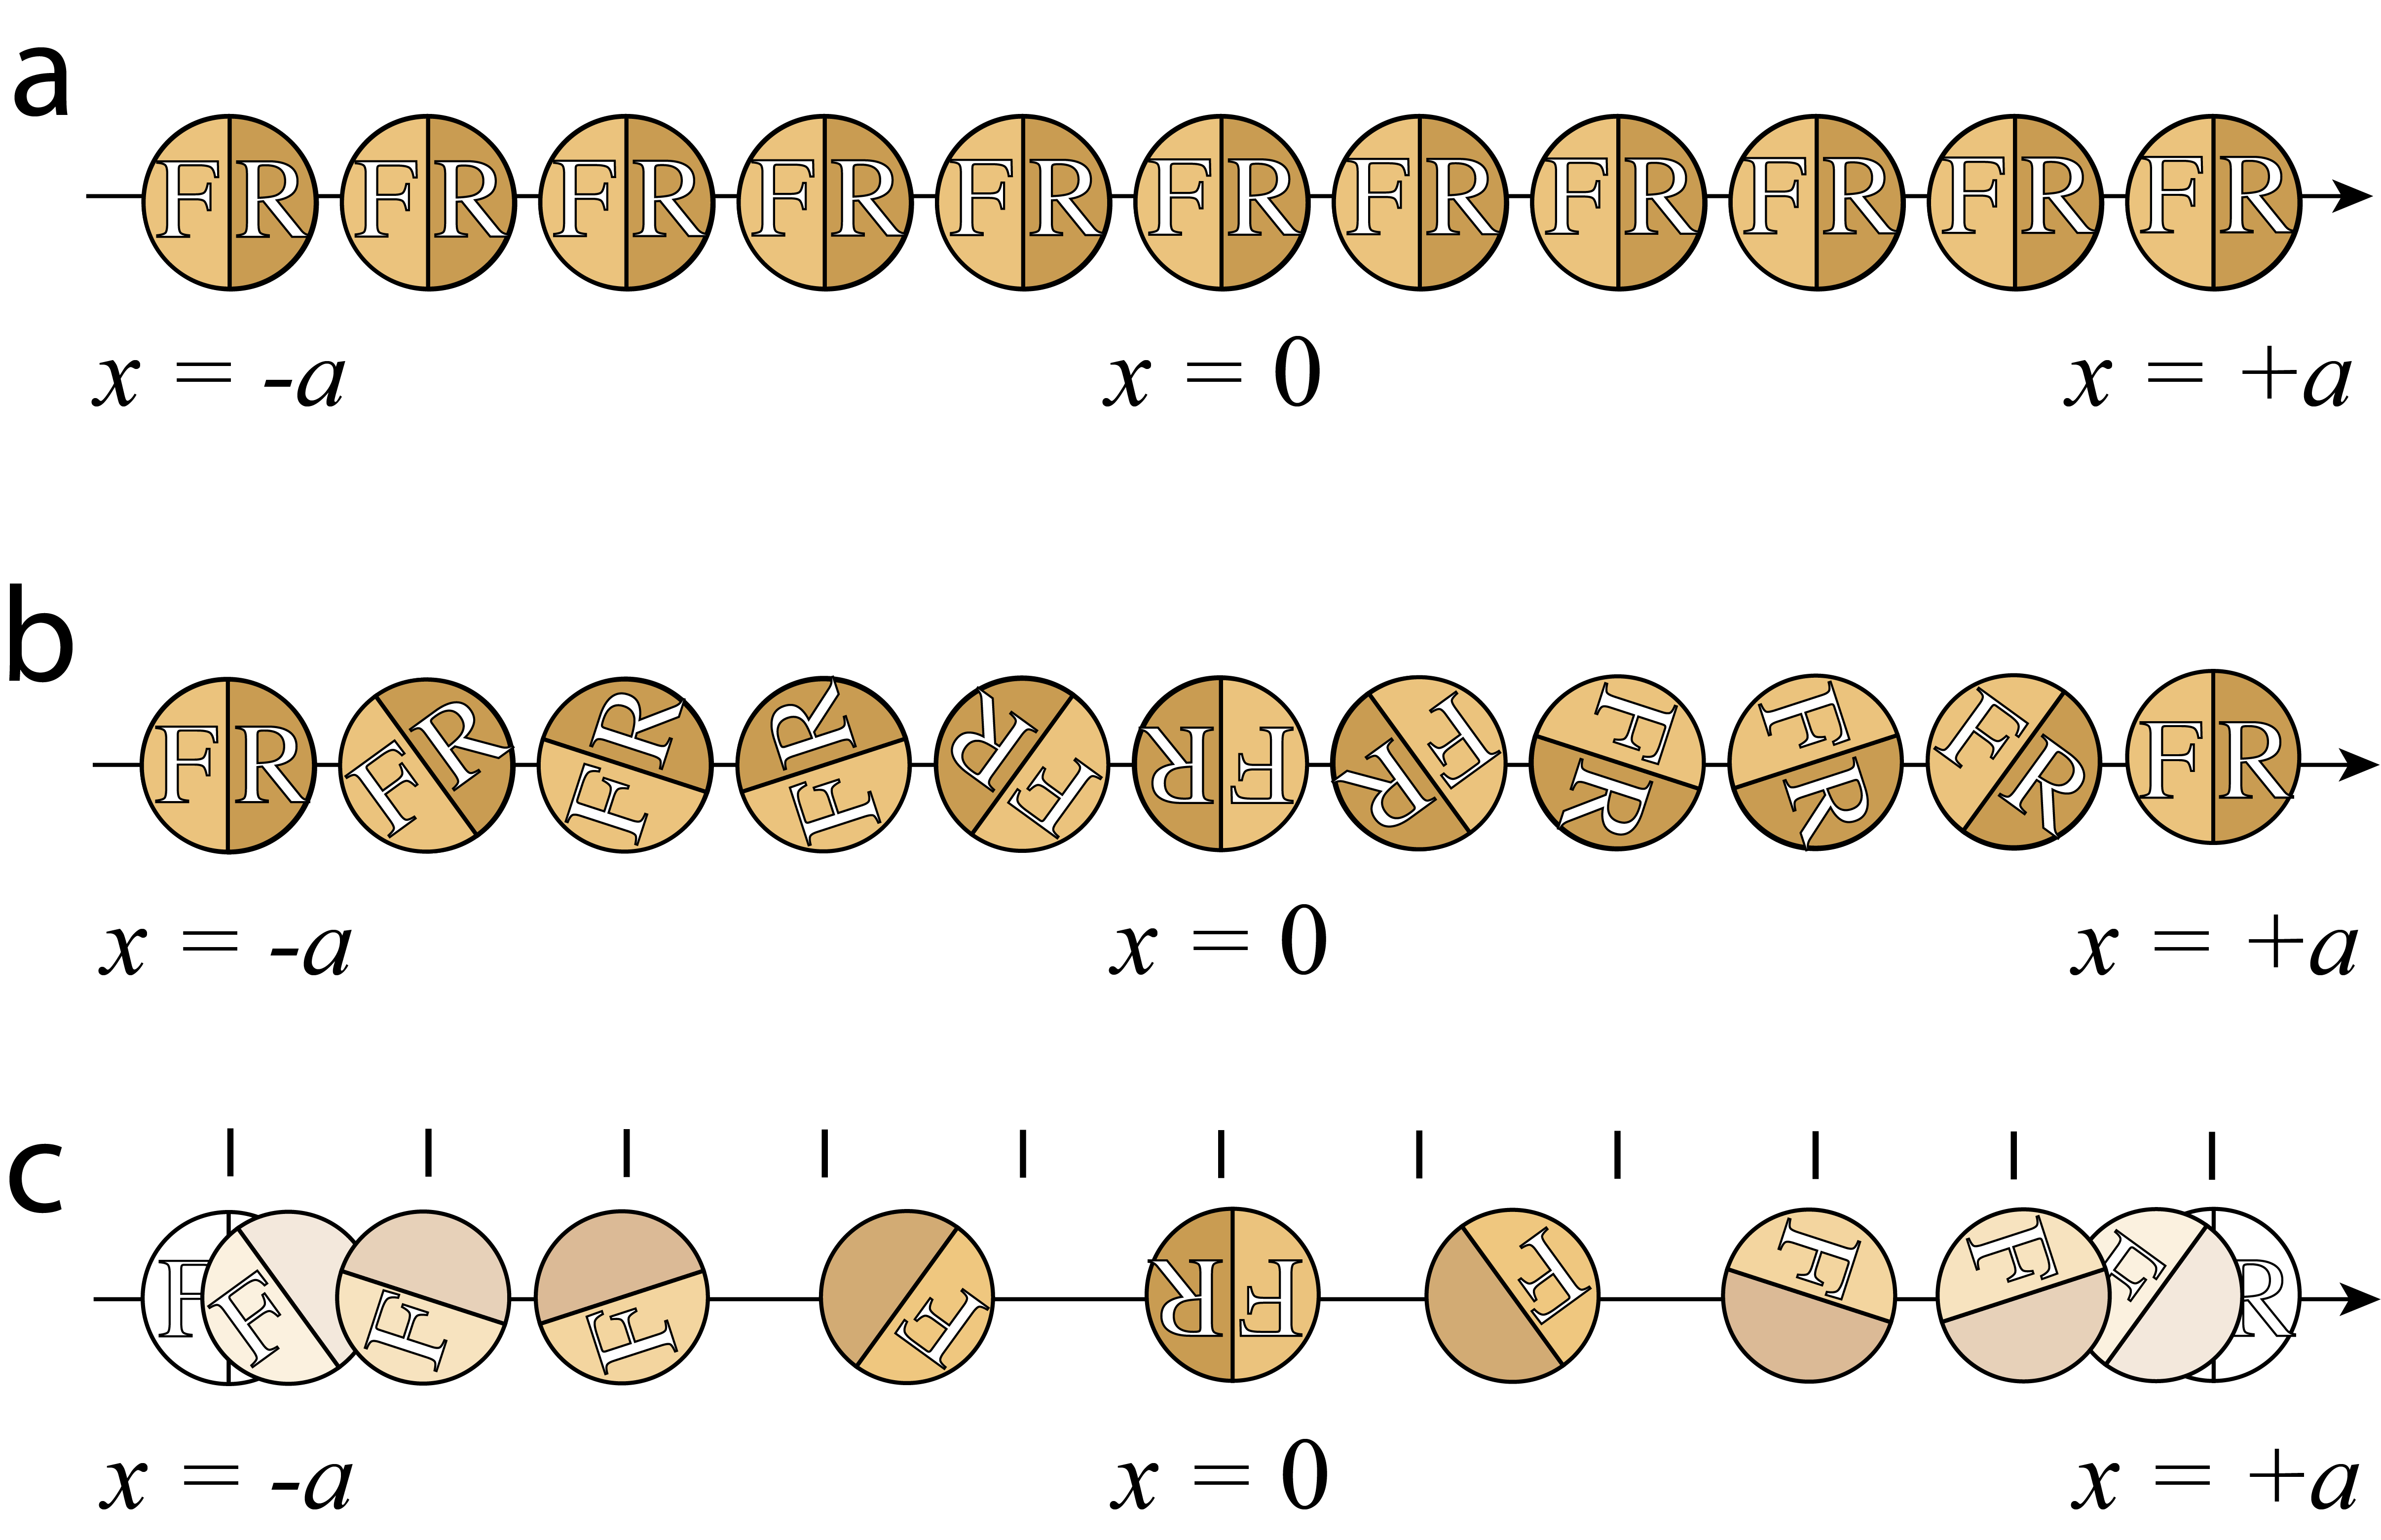
\includegraphics[width=\textwidth]{f-TimeReverce1.png}
    \caption{\justifying Schematic images of spinorial motion and Thomas precession in the 0-Sphere model. (a) Linear uniform motion of $F$-$R$ spheres with constant angular velocity $\omega=0$, representing a zero spin-axis vector in conventional physics. (b) Uniform circular motion through the origin, where $F$-$R$ spheres rotate with constant acceleration, corresponding to angular velocity $\omega=\text{const}$. This represents the conventional spin concept with definite clockwise or counterclockwise rotation, preserving realism in Bell's inequality as described in Eq.~\ref{eq:thomas2}. (c) Harmonic oscillatory motion of $F$-$R$ spheres in both velocity and acceleration, where through reinterpretation of Thomas precession, the spin-axis vector alternates between up and down states depending on the temporal phase, as described by Eq.~\ref{eq:thomas1}. The 0-Sphere model yields an average microscopic Zitterbewegung oscillation velocity approximately $0.04c$. The distance between $x=+a$ and $x=-a$ represents the actual amplitude of the photon sphere's oscillation. The circles represent photon spheres with inherent directional polarity ($F$-$R$), which mediate kinetic energy transport, rather than conventional non-oriented masses. The model introduces these spheres as quantum mechanical entities that manifest both particle-like and wave-like characteristics through their directional polarization and oscillatory motion. The coordinate $x=+a$ represents the initial position where kernel $A$ resides with its rest mass energy, while $x=-a$ represents the endpoint where kernel $B$ is located. The photon sphere mediates energy transfer between these kernels through radiation. In the 0-Sphere model, the photon sphere radius is defined as $r_{\text{photonsphere}} = 2a$, with both kernels $A$ and $B$ existing within this sphere. For clarity of visualization of the 360-degree rotation, the photon sphere is depicted at a reduced scale in these schematic representations.}
    \label{f-TimeReverce1}
\end{figure*}


% Key changes made:
% 1. Changed `figure` to `figure*` to make it span both columns
% 2. Changed `scale=0.20` to `width=\textwidth` to make the figure scale to the full text width



\subsection{Time Reversal in the 0-Sphere Model}

The pendulum representation shown in Fig.~\ref{f-pendlum-spinor} warrants deeper examination in the context of time-reversal symmetry. The reinterpretation of Thomas precession demonstrates that while angular velocity vanishes during uniform linear motion through the origin, it emerges during accelerated motion. This fundamental principle has significant implications for the oscillator model.

To illustrate these implications systematically, consider the progression shown in Fig.~\ref{f-TimeReverce1}. (a) Depicts uniform linear motion without spinorial rotation, where masses maintain constant $F$-$R$ orientation during translation. (b) Shows uniform linear motion incorporating 720-degree spinorial rotation. Neither (a) nor (b) generates angular velocity through Thomas precession due to their uniform motion. (c) Illustrates the mass undergoing simple harmonic acceleration through the origin ($x = 0$). Through deep reinterpretation of Thomas precession, this accelerated motion manifests angular velocity. As the mass traverses from the right endpoint ($x = +a$) to the left endpoint ($x = -a$), while the simple harmonic oscillator phase advances by $\pi$, the $F$-$R$ oriented sphere itself completes a full 360-degree ($2\pi$) rotation. During one complete oscillation cycle, the photon sphere's kinetic energy phase advances by $2\pi$, while the $F$-$R$ sphere undergoes two complete rotations. This relationship provides a novel visualization of the conventional 720-degree spinor periodicity, resolving the long-standing puzzle of why spinors require a $4\pi$ rotation to return to their initial state. The color intensity in (c) correlates with the velocity of the mass: the absence of coloration (white) at $x = \pm a$ indicates zero velocity at these turning points, while the yellow and brown coloring at $x = 0$ represents maximum velocity at the equilibrium position. Moreover, the time-reversal symmetry of spin, expressed as $\mathcal{T}\hat{\boldsymbol{S}}\mathcal{T}^{-1} = -\hat{\boldsymbol{S}}$, naturally corresponds to the spin orientation in (c): spin-up during the initial phase ($0$ to $\pi$) as the mass moves from $+a$ to $-a$, followed by spin-down during the subsequent phase ($\pi$ to $2\pi$), providing a geometric visualization of spin reversal under time reversal.

However, consider the uniform linear motion depicted in Fig.~\ref{f-TimeReverce1}(a), where circular elements progress along a linear path. In this configuration, no angular velocity manifests, rendering this representation insufficient for describing the quantum mechanical behavior of electron spin. This limitation necessitates a more sophisticated model that incorporates the periodic nature of both the kernels and the photon sphere.

As previously established in Eq.~\ref{eq:E0Conservation}, the energy conservation relationship describes the distribution of total energy $E_0$ among different components of the system. A detailed analysis of this equation reveals a critical relationship: kernel $A$ exhibits periodicity in phase $\omega t/2$, while the kinetic energy term of the photon sphere, represented by $\frac{1}{2}\sin^2(\omega t)$, demonstrates periodicity in phase $\omega t$. This doubling of frequency between the kernel components and the photon sphere's kinetic energy term proves fundamental to understanding the quantum mechanical behavior of the system. Equation~\ref{eq:E0Conservation} evokes a more concrete image of the electron: as the photon sphere physically traverses from one endpoint to the other during half a period of simple harmonic motion, it completes one full 360-degree rotation about its axis.

As established in Eq.~\ref{eq:thomas_precession}, the angular velocity arising from Thomas precession reveals a fundamental relationship between phase progression and spin orientation. This mathematical structure indicates that during a phase progression of $\pi$ as the photon sphere travels from $x=+a$ to $x=-a$, the spinor component undergoes a phase advancement of $2\pi$. Fig.~\ref{f-TimeReverce1}(b) illustrates this behavior, depicting one complete rotation of the $F$-$R$-marked circle during a $\pi$ phase progression of the photon sphere.

The well-documented 720-degree periodicity of spinors~\cite{Hestenes1990} finds natural expression in this framework: a $2\pi$ phase progression of the photon sphere corresponds to two complete rotations of the sphere itself. This relationship, illustrated in Fig.~\ref{f-TimeReverce1}(c), provides a novel visualization of spin-1/2 behavior that maintains consistency with both quantum mechanical principles and relativistic constraints~\cite{Dirac1928}.

The representation of harmonic oscillation with directional orientation presented in Fig.~\ref{f-TimeReverce1} offers a unique perspective on spin dynamics, bridging classical and quantum mechanical descriptions while preserving essential mathematical relationships derived from Thomas precession.

This oscillatory behavior, combined with the phase relationships described by Equations~\ref{eq:E0Conservation} and \ref{eq:omega}, provides a comprehensive framework for understanding the emergence of spin in linear harmonic motion. The model resolves the apparent paradox between linear oscillation and angular momentum generation through the geometric phase accumulated during accelerated motion~\cite{Berry1984, Aharonov1987}. This interpretation aligns with modern perspectives on geometric phases in quantum mechanics while maintaining consistency with the principles of special relativity.

The conventional representation of electron spin as continuous rotation, as illustrated in Fig.~\ref{f-barmagnets}, fails to account for the fundamental binary nature of spin states. However, the harmonic oscillator model presented in this study naturally leads to the emergence of spin dichotomy. When a mass undergoes simple harmonic motion through the origin, traditional physics would suggest no angular momentum is generated. This preconception has historically hindered our understanding of spin angular momentum.

The present model demonstrates how the temporal evolution of harmonic oscillation inherently gives rise to two distinct spin states. During the first half-cycle ($0$ to $\pi$), as the oscillator moves from $+a$ to $-a$, the system manifests one spin orientation. In the subsequent half-cycle ($\pi$ to $2\pi$), the time-reversal symmetry of spinors ($\mathcal{T}\hat{\boldsymbol{S}}\mathcal{T}^{-1} = -\hat{\boldsymbol{S}}$) naturally leads to the opposite spin orientation. This bifurcation of spin states emerges not as an imposed condition but as a natural consequence of the oscillator's motion and the inherent properties of spinors under time reversal.

This insight reveals how the quantum mechanical property of spin discreteness can arise from a more fundamental consideration of harmonic motion, providing a bridge between classical and quantum descriptions. The model resolves the long-standing puzzle of spin binary states without invoking additional assumptions, demonstrating that the discrete nature of spin states is intrinsically connected to the temporal evolution of the system.

The photon sphere mechanism in the 0-Sphere model provides a consistent framework for understanding magnetic moment generation and spin state transitions. The relationship between photon sphere velocity and magnetic moment generation suggests potential connections to broader phenomena in quantum systems, warranting further experimental investigation.

A crucial question arises: does the photon sphere, with its radius on the order of the Compton wavelength, avoid exceeding the speed of light during its rotation? Historically, the concept of an electron with finite size has been rejected due to the superluminal velocities it would necessitate. In the following subsection, we will review this historical context and demonstrate how the 0-Sphere model, with its prediction that Zitterbewegung oscillation velocity is approximately $0.04c$, provides a mathematical framework that remains consistently below the speed of light.


\subsection{Magnetization Dynamics and Phase Transition in the Oscillator Model}
\label{MagnetizationDynamicsAnd}

A critical examination of the transition from Fig.~\ref{f-pendlum-spinor}(c) to (d) reveals a fundamental challenge in the preservation of forward orientation during oscillation. If the mass were to reverse its orientation at the endpoints through continuous rotation, it would necessitate a classical magnetic pole reversal process analogous to that shown in Fig.~\ref{f-barmagnets}. Such a reversal would require intermediate orientations, similar to the bar magnets positioned at 3 o'clock and 9 o'clock in Fig.~\ref{f-barmagnets}, to transition between the 12 o'clock and 6 o'clock positions.

An instantaneous $F$-$R$ reversal would violate special relativity's prohibition of superluminal motion~\cite{Einstein1905}. This constraint is analogous to the classical requirement that flipping a coin from heads to tails, even at the oscillation endpoints where velocity vanishes, necessitates a finite time interval. The 0-Sphere model addresses this apparent paradox through the photon sphere mechanism revealed in Fig.~\ref{f-TimeReverce1}(c).

The photon sphere in this model mediates kinetic energy transport and exhibits unique behavior at the endpoints ($x = \pm a$) where the oscillator velocity vanishes. At these points, the photon sphere velocity reaches zero, leading to a nullification of magnetic effects. This state is analogous to the Meissner effect in superconductivity where photons, acquiring effective mass, exclude magnetic flux lines~\cite{Cohen1997}. The absence of coloration (white circles) at the endpoints in Fig.~\ref{f-TimeReverce1}(c) signifies this vanishing the photon sphere velocity and corresponding zero magnetic moment.



\begin{figure*}[t!]
    \centering
    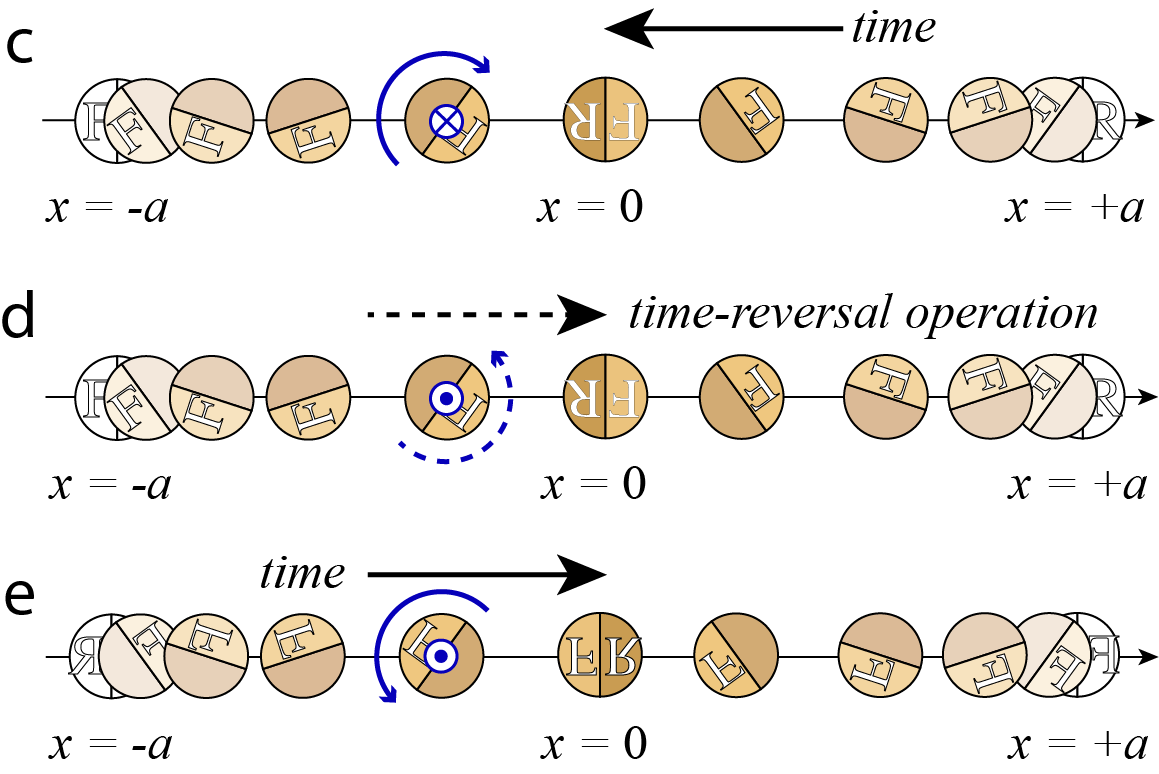
\includegraphics[width=\textwidth]{f-TimeReverce2.png}
    \caption{\justifying Time-reversal symmetry demonstration in the 0-Sphere model. Panel (c) represents temporal phase 0 to $\pi$ corresponding to the state $\hat{\boldsymbol{S}}$, panel (d) shows time-reversed state ($\pi$ to 0) representing $\mathcal{T}\hat{\boldsymbol{S}}\mathcal{T}^{-1}$, and panel (e) depicts phase $\pi$ to 2$\pi$ showing $-\hat{\boldsymbol{S}}$. Blue arrows indicate the spin axial vector direction. The $F$-$R$ mirror reflection in panel (e) illustrates the spinorial characteristic of mirror image inversion during directional reversal, providing a geometric visualization of spin's pseudovectorial nature (see Section~\ref{subsec:PseudovectorNature}).  In panel (c), the circle rotates clockwise, though this choice is arbitrary and has no mathematical significance - counterclockwise rotation would be equally valid. The $x$-axis in the figure represents the spatial trajectory of the electron's Zitterbewegung oscillation, showing its motion from $x=+a$ to $x=-a$ and back to $x=+a$. While the electron traverses the $x$-coordinate, the $F$-$R$ circle's spin axis vector maintains its orientation in the direction of motion. For clarity of visualization, we have taken the $z$-axis to be perpendicular to the page (pointing towards the viewer) to better illustrate the spin axis vector. In reality, the photon sphere maintains its spin axis vector parallel to the direction of motion along the $x$-axis while undergoing Larmor precession. This precession, though not explicitly shown in the figure for simplicity, is an essential feature of the electron's motion. The preservation of spin orientation relative to motion direction, combined with the $F$-$R$ mirror reflection, demonstrates how the model naturally incorporates the fundamental transformation properties of pseudovectors under spatial inversion.}
    \label{f-TimeReverce2}
\end{figure*}



Time-reversal symmetry demonstration in the 0-Sphere model (Fig.~\ref{f-TimeReverce2}) provides a comprehensive visualization of spin state transitions. Panel (c) represents phase 0 to $\pi$ corresponding to the state $\hat{\boldsymbol{S}}$, where the circle rotates clockwise. This choice of rotation direction is arbitrary and has no mathematical significance - counterclockwise rotation would be equally valid. Panel (d) shows the time-reversed state ($\pi$ to 0), representing $\mathcal{T}\hat{\boldsymbol{S}}\mathcal{T}^{-1}$, demonstrating how the spin orientation transforms under time reversal. Panel (e) depicts phase $\pi$ to 2$\pi$ showing $-\hat{\boldsymbol{S}}$, with the $F$-$R$ mirror reflection illustrating the spinorial characteristic of mirror image inversion during directional reversal.

The $x$-axis in the figure represents the spatial trajectory of the electron's Zitterbewegung oscillation, showing its motion from $x=+a$ to $x=-a$ and back to $x=+a$. While the electron traverses the $x$-coordinate, the $F$-$R$ circle's spin axis vector (indicated by blue arrows) maintains its orientation in the direction of motion. For clarity of visualization, we have taken the $z$-axis to be perpendicular to the page (pointing towards the viewer) to better illustrate the spin axis vector. In reality, the photon sphere maintains its spin axis vector parallel to the direction of motion along the $x$-axis while undergoing Larmor precession, though this precession is not explicitly shown in the figure for simplicity.

The notion of massive, stationary photons at the endpoints aligns with established quantum mechanical observations in superconducting states. This framework provided by the closed algebraic equations of the 0-Sphere model offers a consistent interpretation of the experimentally observed binary nature of spin states without contradicting fundamental physical principles. The relationship between the photon sphere velocity and magnetic moment generation suggests potential connections to broader phenomena in quantum systems, warranting further experimental investigation.





\subsection{Interpretation of Quantum Entanglement States Through Temporal Phase}\label{subsec:quantum_entanglement}

The quantum entanglement state represents a state where two electrons take states (c) and (e) respectively, as shown in Fig. 5 (\ref{f-TimeReverce2}). When single electron rest masses are placed in two kernels $A$ and $B$ and the pendulums begin to oscillate, the two simple pendulums interact alternately. This state constitutes quantum entanglement, where each pendulum alternates between $\hat{\boldsymbol{S}}$ and $-\hat{\boldsymbol{S}}$ states in temporal phase. This represents the alternating state of up and down spins, and even when the two electrons are separated remotely, as long as they oscillate in the same period and direction—that is, in a coherent state—each single electron periodically alternates between up and down spins without requiring Einstein's ``spooky action at a distance.'' The up and down spins are then revealed upon measurement. Through the progression of temporal phase, the two electrons alternately transition between $\hat{\boldsymbol{S}}$ and $-\hat{\boldsymbol{S}}$ states. Therefore, each spin is not predetermined, which constitutes a violation of realism. This provides a basis for accepting the violation of realism (where spin is not predetermined) without violating the locality in Bell's inequality.

Therefore, the energy state of the quantum entanglement state in the 0-Sphere model can be expressed as follows:
\begin{equation}
\label{eq:2E0}
\begin{split}
2E_0 = & E_0\left(\cos^4\left(\frac{\omega_{e1} t}{2}\right) + \sin^4\left(\frac{\omega_{e1} t}{2}\right) + \frac{1}{2}\sin^2(\omega_{e1} t)\right) \\
       & + E_0\left(\cos^4\left(\frac{\omega_{e2} t}{2} + \frac{2\pi}{2} \right) + \sin^4\left(\frac{\omega_{e2} t}{2} + \frac{2\pi}{2} \right) \right. \\
       & \left. + \frac{1}{2}\sin^2(\omega_{e2} t + \pi)\right)
\end{split}
\end{equation}

Quantum entanglement requires that the angular momenta of the two electrons must be identical, meaning $\omega_{e1}=\omega_{e2}$. When the phases $\omega_{e1} \neq \omega_{e2}$, the periodicity of alternation between $\hat{\boldsymbol{S}}$ and $-\hat{\boldsymbol{S}}$ states becomes inconsistent, leading to decoherence. The expression $\frac{2\pi}{2}$ is deliberately used without simplification in the $\cos^4$ and $\sin^4$ terms to emphasize that these terms represent spinorial oscillators. This equation represents the state of two entangled single electrons, where the total energy $2E_0$ remains constant regardless of temporal phase changes, thus satisfying the law of energy conservation.

Separating entangled electrons to remote locations means maintaining equal $\omega_{e1}$ and $\omega_{e2}$ while physically separating them. Both electrons continue to alternate between spin-up and spin-down states at the same frequency. Therefore, when one electron is measured and found to be in state $\hat{\boldsymbol{S}}$, the other electron's state is determined to be $-\hat{\boldsymbol{S}}$ without requiring any``spooky action at a distance.''


\subsection{Pseudovectorial Nature of Spin \\in the 0-Sphere Model}
\label{subsec:PseudovectorNature}

The behavior of the photon sphere during harmonic oscillation provides a natural geometric interpretation of spin's pseudovectorial nature. While the FR circle undergoes mirror reflection during direction reversal, the preservation of clockwise rotation demonstrates how spin angular momentum transforms differently from polar vectors under coordinate inversion. This characteristic aligns with the mathematical properties of pseudovectors, where \( \hat{\boldsymbol{S}} \rightarrow \hat{\boldsymbol{S}} \) under parity transformation, distinguishing spin from conventional polar vectors \( \vec{r} \rightarrow -\vec{r} \).

Moreover, this inherent pseudovectorial behavior manifests in the model's treatment of time-reversal symmetry. The photon sphere's preservation of rotational direction relative to its motion, even after spatial inversion, naturally explains why spin angular momentum behaves as a pseudovector rather than a polar vector. This geometric property emerges organically from the model's structure rather than being imposed as an additional constraint, providing a natural framework for understanding the transformation properties of spin angular momentum.



\subsection{Relativistic Limitations and the 0-Sphere Model}
\label{sec:rel_limit_0sphere}

\subsubsection{Historical Context: Relativistic Limitations \\of Classical Electron Spin}
\label{subsec:hist_context}

The classical interpretation of electron spin as a rotating sphere encountered a fundamental contradiction with special relativity theory~\cite{Tomonaga1997}. This limitation emerged from a straightforward calculation of the equatorial velocity of a hypothetical spinning electron. The calculation proceeds from the known quantum mechanical spin angular momentum of the electron, $S = \hbar/2$, and attempts to interpret it as classical rotational motion.

For a spherical electron with classical radius $r_e = e^2/mc^2$, the moment of inertia $I$ is given by:

\begin{equation}
\label{eq:moment_inertia}
I = \frac{2}{5}mr_e^2
\end{equation}

The angular velocity $\omega$ can be derived from the spin angular momentum relation:

\begin{equation}
\label{eq:angular_velocity}
S = \frac{\hbar}{2} = I\omega
\end{equation}

Substituting Equation \ref{eq:moment_inertia} into \ref{eq:angular_velocity} yields:

\begin{equation}
\label{eq:omega_calc}
\omega = \frac{5\hbar}{4mr_e^2}
\end{equation}

The equatorial velocity $v$ is then:

\begin{equation}
\label{eq:equatorial_velocity}
v = \omega r_e = \frac{5\hbar}{4mr_e}
\end{equation}

When numerical values are inserted ($\hbar = 1.05 \times 10^{-34}~\mathrm{J \cdot s}$, $m = 9.11 \times 10^{-31}~\mathrm{kg}$, $r_e = 2.82 \times 10^{-15}~\mathrm{m}$), the equatorial velocity becomes:

\begin{equation}
\label{eq:velocity_result_corrected}
v \approx 170c
\end{equation}

This result, exceeding the speed of light by more than two orders of magnitude, further demonstrates the incompatibility between classical rotation and quantum spin~\cite{Ohanian1986}.



\subsubsection{The Velocity of Electrons in the Bohr Model:\\ A Classical Paradox}
\label{subsec:bohr_velocity}

The Bohr model, a cornerstone of early quantum theory, provides an illustrative, albeit simplified, framework to understand the motion of electrons in hydrogen-like atoms. In this model, electrons are assumed to revolve around the nucleus in circular orbits, with their motion governed by the quantization of angular momentum. While the Bohr model offers valuable insights into atomic spectra and the quantization of energy levels, it also presents intriguing challenges, particularly when examining the velocity of electrons in their designated orbits.

The velocity of an electron in the Bohr model can be derived by considering the balance of forces acting on the electron. The centripetal force required for circular motion is provided by the Coulomb attraction between the positively charged nucleus and the negatively charged electron. The balance of forces leads to the equation:

\begin{equation}
\frac{m v^2}{r} = \frac{Z e^2}{4 \pi \epsilon_0 r^2},
\label{eq:centripetal_force}
\end{equation}
where \( m \) is the mass of the electron, \( v \) is its orbital velocity, \( r \) is the radius of the orbit, \( Z \) is the atomic number (with \( Z = 1 \) for hydrogen), \( e \) is the elementary charge, and \( \epsilon_0 \) is the permittivity of free space.

The quantization of angular momentum in the Bohr model stipulates that:

\begin{equation}
m v r = n \hbar,
\label{eq:angular_momentum}
\end{equation}
where \( n \) is the principal quantum number and \( \hbar \) is the reduced Planck constant. By solving Equation \ref{eq:centripetal_force} and Equation \ref{eq:angular_momentum}, one can express the velocity \( v \) of the electron as:

\begin{equation}
v = \frac{Z e^2}{4 \pi \epsilon_0 \hbar}.
\label{eq:bohr_velocity}
\end{equation}

Substituting the known physical constants for a hydrogen atom (\( Z = 1 \)), we obtain:

\begin{equation}
v = \alpha c,
\label{eq:bohr_velocity_alpha}
\end{equation}
where \( \alpha \) is the fine-structure constant, approximately equal to \( 1/137 \), and \( c \) is the speed of light in a vacuum. Thus, the electron in the ground state of the hydrogen atom moves at roughly \( 1\% \) of the speed of light.

An apparent paradox arises when extending this reasoning to highly charged nuclei or when interpreting classical analogs to quantum spin. For example, in the classical depiction of spin angular momentum, attempts to ascribe a rigid spherical rotation to the electron lead to surface velocities exceeding the speed of light. Such results are inconsistent with the tenets of special relativity, which prohibit any physical object or signal from traveling faster than \( c \)~\cite{Einstein1905}. In the Bohr model context, the issue becomes pronounced for high-\( Z \) nuclei, where \( v \propto Z \), implying that relativistic corrections become increasingly significant.

The comparison of the Bohr velocity expression with the classical spin surface velocity illustrates a conceptual divergence. While the Bohr model velocity remains subluminal for hydrogen, the rigid-body interpretation of electron spin leads to calculated surface velocities like \( 137c \) or \( 170c \), as discussed in Subsection~\ref{sec:rel_limit_0sphere}. These estimates, rooted in classical mechanics, are physically inadmissible because they violate the relativistic invariance of the speed of light~\cite{Tomonaga1997, Ohanian1986}.

While the Bohr model provides a foundational understanding of atomic structure, its classical underpinnings necessitate careful reinterpretation when applied to relativistic or quantum mechanical ~\cite{Dirac1928}. The velocity derived for electrons in hydrogen-like atoms, approximately \( \alpha c \), exemplifies the utility and limitations of the model. Furthermore, comparisons with classical interpretations of spin underscore the necessity of modern quantum theories that transcend classical analogies. The rejection of superluminal surface velocities, as derived from classical spin analogies, reaffirms the fundamental principles of relativity and highlights the intricate interplay between classical and quantum perspectives.



\subsubsection{Interpretations in the 0-Sphere Model}
The 0-Sphere model presents a distinct departure from conventional electron representations. Rather than maintaining an ambiguous description that merely acknowledges both particle and wave characteristics, the model provides a precise energetic allocation for these dual properties. The single electron in the 0-Sphere model manifests both particle and wave attributes through a well-defined energy distribution mechanism, which can be expressed as:

\begin{equation}
E_{total} = E_{kernel} + E_{kinetic}
\label{eq:energy_distribution}
\end{equation}
where $E_{kernel}$ represents the rest mass energy distributed between kernels $A$ and $B$, and $E_{kinetic}$ denotes the converted motion energy.

The kernels $A$ and $B$, representing distinct manifestations of rest mass, undergo phase-dependent dissolution. While the term ``dissolution'' warrants careful consideration, it effectively describes the temporal transformation process. The model postulates that kernel $A$ possesses finite dimensions, a necessary condition for temporal phase-dependent dissolution. This finite size requirement emerges from the mathematical constraint that a point-like kernel would preclude dissolution within finite time parameters.

Historically, the concept of finite electron size has been algebraically rejected due to rotational considerations~\cite{MacGregor1992}. As discussed in the previous subsection, a rigid body interpretation of finite electron size necessitates either angular momentum complications or superluminal surface velocities, both of which violate relativistic constraints~\cite{Barut1994}. The 0-Sphere model circumvents these limitations by eliminating rotational motion entirely. Instead, the kernels undergo dissolution within finite time intervals. The Two-Photon Exchange (TPE) energy possessed by the kernels completely converts to kinetic energy according to Eq. \ref{eq:E0Conservation}.

Although the kernels themselves do not rotate, the model proposes the existence of a real the photon sphere surrounding the single electron, with a radius on the order of the Compton wavelength. Kernels $A$ and $B$ exist within this photon sphere. Consequently, the kinetic energy radiated from kernel $A$ is propagated through these physically existing photons, aligning with conventional physical understanding of radiation transport through photons~\cite{Cohen1997}. This mechanism exhibits conceptual parallels with solar radiation pressure transporting energy to Earth, though with a fundamental distinction: whereas solar radiation represents an external driving force, the 0-Sphere model describes an internally driven system where the source of radiation pressure resides within the photon sphere itself. This intrinsic oscillation mechanism differentiates the electron's behavior in the 0-Sphere model from externally driven radiation phenomena~\cite{Jackson1998}.

Given that the electron's Zitterbewegung moves at approximately $0.04c$, the subsequent subsection will demonstrate that even if this photon sphere rotates, its equatorial velocity remains below the speed of light. The physical implications of this photon sphere rotation lie beyond the scope of the present investigation and warrant future examination. This formulation maintains consistency with quantum electrodynamics while avoiding the complications associated with classical rotational models~\cite{Hestenes1990}.

The key innovative aspects presented in this subsubsection can be summarized as follows:

\begin{enumerate}

\item \textbf{Internal Radiation Drive:} The model proposes an internally driven radiation mechanism that generates the electron's Zitterbewegung motion. This mechanism, distinct from external radiation phenomena, explains the origin of the oscillatory motion as an inherent property of the electron's structure, while maintaining consistency with established quantum electrodynamics principles. The internal radiation pressure serves as the driving force for the characteristic trembling motion (Zitterbewegung) occurring at approximately $0.04c$.

\item \textbf{Precise Energy Allocation:} The model provides a quantitative framework for the distribution of energy between particle and wave characteristics, replacing traditional qualitative descriptions.

\item \textbf{Improve Rest Mass Structure:} The introduction of kernels $A$ and $B$ as distinct manifestations of rest mass, with a phase-dependent dissolution mechanism, offers a new perspective on electron structure.

\item \textbf{Introduction of The Photon Sphere:} The model introduces the photon sphere with a radius on the Compton wavelength scale, which provides a physical mechanism for energy propagation. This photon sphere, having dimensions on the order of the Compton wavelength, differs from conventional electron models. The concept enables analysis of kinetic energy management through spherical harmonics, offering a mathematical framework for understanding the spatial distribution and dynamics of energy transport within the electron structure~\cite{Arfken2012}. This photon sphere as a component of electron structure presents a new perspective in quantum electrodynamics.

\item \textbf{Non-rotational Solution:} The model resolves the historical paradox of finite electron size by eliminating rotation entirely, replacing it with a dissolution-based energy conversion process.

\end{enumerate}

These innovations collectively constitute a self-consistent framework that addresses longstanding challenges in electron modeling while maintaining compatibility with both relativistic constraints and quantum mechanical principles. The implications of this framework, particularly regarding the photon sphere's behavior, suggest promising directions for future investigation.



\vfill


\subsubsection{The 0-Sphere Electron Model and Zitterbewegung:\\ A Relativistic Perspective}
\label{subsec:0sphere_model_relativistic}

In previous work~\cite{Hanamura2023}, it was demonstrated that Zitterbewegung can occur in a single electron through a reinterpretation of Dirac equation's negative energy solutions. Rather than interpreting these negative energy solutions as antimatter states, they correspond to the kernel pairs in the 0-Sphere model. This interpretation enables Zitterbewegung to manifest in single electrons, as predicted by the Dirac equation.

Building on this foundation, the relationship between the electron's anomalous magnetic moment and Lorentz contraction during Zitterbewegung oscillation was established through the equation:
\begin{equation}
\label{eq:lorentz_anomalous}
\sqrt{1 - \frac{v^2}{c^2}} = \frac{1}{1 + \frac{1}{\sqrt{2}} a^{\text{exp}}_{\text{e}}}
\end{equation}
where $a^{\text{exp}}_{\text{e}} = 0.001\,159\,652\,180\,59\,(13)$ is the experimentally measured anomalous magnetic moment of the electron~\cite{Fan}. Solving this equation for $v$ yields:
\begin{equation}
\label{eq:zitter_velocity}
v_{\text{electron}}^{\gamma^{*}} \fallingdotseq 0.04047197635 \times c
\end{equation}

The 0-Sphere model provides a self-consistent framework for analyzing electron spin dynamics without violating relativistic constraints. Consider a spherical object moving linearly from point A ($x = +a$) to point B ($x = -a$) at the calculated Zitterbewegung velocity of approximately 4\% of the speed of light, $v_{linear} = 0.04c$. The total distance covered during this motion is set to the electron's Compton wavelength, $\lambda_c = h/mc$, which corresponds to the amplitude of Zitterbewegung predicted by the Dirac equation~\cite{Hestenes1990}. Additionally, the sphere's radius is set equal to $\lambda_c$, encapsulating the characteristic spatial scale of quantum mechanical oscillations.

The system parameters can thus be summarized as follows:
\begin{equation}
\label{eq:system_params_corrected}
\begin{aligned}
v_{linear} &= 0.04c, \\
2a &= \lambda_c, \\
r &= \lambda_c.
\end{aligned}
\end{equation}

The time required for the sphere to traverse this distance at the given linear velocity is calculated as:
\begin{equation}
\label{eq:transit_time_corrected}
T = \frac{\lambda_c}{v_{linear}} = \frac{\lambda_c}{0.04c} = \frac{h}{mc^2 \cdot 0.04} = \frac{25h}{mc^2}.
\end{equation}

During this interval, the sphere completes one full rotation ($2\pi$ radians). The tangential velocity at the equator, arising from this rotational motion, is determined by:
\begin{equation}
\label{eq:tangential_velocity_corrected}
v_{tangential} = \omega r = \frac{2\pi r}{T} = \frac{2\pi \lambda_c}{\frac{25h}{mc^2}} = \frac{2\pi \cdot mc^2 \cdot \lambda_c}{25h}.
\end{equation}

Substituting $\lambda_c = h/mc$ simplifies the expression:
\begin{equation}
v_{tangential} = \frac{2\pi h/mc \cdot mc^2}{25h} = \frac{2\pi c}{25} \approx 0.08\pi c.
\end{equation}

The total velocity at the equator is the vector sum of the linear velocity and the tangential velocity. Using the Pythagorean theorem, this is given by:
\begin{equation}
\label{eq:total_velocity_corrected}
v_{total} = \sqrt{v_{linear}^2 + v_{tangential}^2}.
\end{equation}

Substituting $v_{linear} = 0.04c$ and $v_{tangential} = 0.08\pi c$, we find:
\begin{equation}
\begin{aligned}
v_{total} &= c\sqrt{(0.04)^2 + (0.08\pi)^2} \\ &
\approx c\sqrt{0.0016 + 0.0632} \\ &
\approx c\sqrt{0.0648}.
\end{aligned}
\end{equation}

Numerical evaluation yields:
\begin{equation}
v_{total} \approx 0.2547c.
\end{equation}

To further validate the relativistic consistency of this model, we now consider the maximum instantaneous velocity predicted for Zitterbewegung. The relationship between Lorentz contraction and the anomalous magnetic moment can be expressed without using the root-mean-square (RMS) value:
\begin{equation}
\label{eq:lorentz_direct}
\frac{L}{L_0} = \frac{1}{1 + a^{\text{exp}}_{\text{e}}}
\end{equation}
This equation yields the theoretical maximum velocity of the photon sphere's motion. Compared to Eq.~\ref{eq:lorentz_anomalous}, the $1/\sqrt{2}$ term is absent from the denominator, resulting in a higher velocity than that derived from Eq.~\ref{eq:lorentz_anomalous}. According to~\cite{Hanamura2023}, solving this equation gives the maximum velocity:
\begin{equation}
\label{eq:max_velocity}
v_{max} = \beta_{max}c = 0.048117317159c
\end{equation}

This value represents the instantaneous maximum velocity, in contrast to the RMS-derived average velocity of approximately $0.04c$ discussed earlier.

Even at this maximum velocity, the linear and rotational contributions remain within relativistic limits. Using the same framework for calculating the total velocity, we substitute $v_{linear} = 0.048117317159c$ and $v_{tangential} = 0.08\pi c$:
\begin{equation}
v_{total, max} = c\sqrt{(0.048117317159)^2 + (0.08\pi)^2}.
\end{equation}

Performing the computation:
\begin{equation}
\begin{aligned}
v_{total, max} &= c\sqrt{0.002315 + 0.0632} \\ &
= c\sqrt{0.065515} \\ &
\approx 0.256c.
\end{aligned}
\end{equation}

Thus, even when incorporating the maximum velocity of Zitterbewegung as predicted by the model, the equatorial velocity remains approximately $0.256c$, well below the relativistic limit. 

This analysis demonstrates that the 0-Sphere model avoids the unphysical predictions of classical spin interpretations, such as velocities exceeding the speed of light. Both the average and maximum velocities predicted for Zitterbewegung are consistent with special relativity and further affirm the model's robustness in describing electron dynamics within quantum mechanical and relativistic frameworks.



\section{Conclusion}
\label{sec:conclusion}

The present study has established a fundamental connection between electron spin states and periodic variations through the analysis of Thomas precession in accelerated motion. The algebraic derivation demonstrates that spin states emerge from dynamic processes rather than existing as predetermined properties, providing new insights into the nature of quantum mechanical systems.

The natural emergence of spin's pseudovectorial properties in the 0-Sphere model provides a geometric foundation for understanding quantum phenomena. The model's ability to explain how \( \hat{\boldsymbol{S}} \rightarrow \hat{\boldsymbol{S}} \) under parity transformation while preserving the time-reversal symmetry \( \mathcal{T}\hat{\boldsymbol{S}}\mathcal{T}^{-1} = -\hat{\boldsymbol{S}} \) demonstrates its consistency with fundamental quantum mechanical principles. This geometric interpretation bridges the gap between classical intuition and quantum mechanical observations, particularly in explaining the discrete nature of spin states and their transformation properties.

The reinterpretation of Thomas precession has led to several significant findings. First, the 0-Sphere model naturally explains the quantization of spin angular momentum to $\hbar/2$, through the mathematical structure revealed in Equation~\ref{eq:omega}, where the double angle term emerges from the outer product operation. This result bridges the historical gap between classical and quantum mechanical descriptions of angular momentum.

A significant advancement in the understanding of spin dynamics may arise from the harmonic oscillator framework illustrated in Fig.~\ref{f-TimeReverce1}. This model elucidates how uniform acceleration through the origin—traditionally regarded as incapable of generating angular momentum—can give rise to spin angular momentum when interpreted through the lens of a redefined Thomas precession. By incorporating this reinterpretation, the framework offers a novel perspective on the mathematical foundations of the $4\pi$ periodicity characteristic of spin-$\frac{1}{2}$ particles.

The temporal evolution of the system naturally gives rise to spin dichotomy, as shown in Section \ref{sec:ElectronSpinReinterpreted}. Through closed algebraic equations, this study demonstrates that spin states emerge dynamically through phase progression. The mathematical framework reveals how time-reversal symmetry of spinors combines with the 720-degree periodicity of harmonic oscillation to establish a rigorous basis for spin state alternation. Specifically, during one oscillation cycle, the phase progression from $0$ to $\pi$ corresponds to spin-up, while the subsequent progression from $\pi$ to $2\pi$ corresponds to spin-down.

This framework provides significant insights into Bell's inequality violation. Most notably, our analysis reveals that quantum entanglement can be understood through temporal phase progression, where two electrons in states $\hat{\boldsymbol{S}}$ and $-\hat{\boldsymbol{S}}$ respectively (as shown in Fig.~\ref{f-TimeReverce2}) maintain their correlation through coherent oscillations rather than ``spooky action at a distance.'' This formulation through closed algebraic equations provides mathematical evidence supporting the violation of realism rather than locality in quantum mechanics, while maintaining consistency with special relativity.

Furthermore, the relativistic analysis presented in Section \ref{sec:Discussion} demonstrates that the model avoids the historical paradox of superluminal surface velocities in classical electron models. Even at maximum Zitterbewegung velocity, the total velocity remains well below the speed of light, ensuring compatibility with special relativity.

The 0-Sphere model's introduction of the photon sphere with radius on the order of the Compton wavelength provides a novel mechanism for understanding energy transport in quantum systems. This framework maintains consistency with quantum electrodynamics while avoiding the complications associated with classical rotational models. These findings collectively suggest a new direction in quantum foundations research, offering a mathematical framework that naturally accommodates both the discrete nature of quantum phenomena and the continuous evolution described by the Schrödinger equation. Future investigations may explore the implications of this framework for quantum entanglement and the development of quantum technologies.



\bibliographystyle{plain}
\begin{thebibliography}{99}

\bibitem{Bell1964}
Bell, J. S.,
\textit{On the Einstein Podolsky Rosen Paradox},
Physics,
\textbf{1}(3), 195-200 (1964).
\href{https://doi.org/10.1103/PhysicsPhysiqueFizika.1.195}{doi:10.1103/PhysicsPhysiqueFizika.1.195}

\bibitem{Aspect1982}
Aspect, A., Grangier, P., \& Roger, G.,
\textit{Experimental Realization of Einstein-Podolsky-Rosen-Bohm Gedankenexperiment: A New Violation of Bell's Inequalities},
Physical Review Letters,
\textbf{49}(2), 91-94 (1982).
\href{https://doi.org/10.1103/PhysRevLett.49.91}{doi:10.1103/PhysRevLett.49.91}

\bibitem{Zeilinger2018}
Zeilinger, A.,
\textit{Quantum Entanglement is Independent of Space and Time},
Nature Physics,
\textbf{14}(9), 893-895 (2018).
\href{https://doi.org/10.1038/s41567-018-0297-3}{doi:10.1038/s41567-018-0297-3}

\bibitem{Gerlach1922}
Gerlach, W., \& Stern, O.,
\textit{Der experimentelle Nachweis der Richtungsquantelung im Magnetfeld},
Zeitschrift für Physik,
\textbf{9}(1), 349-352 (1922).
\href{https://doi.org/10.1007/BF01558878}{doi:10.1007/BF01558878}

\bibitem{EPR1935}
Einstein, A., Podolsky, B., \& Rosen, N.,
\textit{Can Quantum-Mechanical Description of Physical Reality Be Considered Complete?},
Physical Review,
\textbf{47}(10), 777-780 (1935).
\href{https://doi.org/10.1103/PhysRev.47.777}{doi:10.1103/PhysRev.47.777}

\bibitem{Hanamura2023}
S. Hanamura, Redefining Electron Spin and Anomalous Magnetic Moment Through Harmonic Oscillation and Lorentz Contraction, Zenodo (2023), \href{https://doi.org/10.5281/zenodo.17764997}{doi:10.5281/zenodo.17764997}. [Originally: \href{https://vixra.org/abs/2309.0047}{viXra:2309.0047}]

\bibitem{Hanamura2018}
S. Hanamura, A Model of an Electron Including Two Perfect Black Bodies, Zenodo (2018), \href{https://doi.org/10.5281/zenodo.16759284}{doi:10.5281/zenodo.16759284}. [Originally: \href{http://vixra.org/abs/1811.0312}{viXra:1811.0312}]

\bibitem{pauli1946}
Pauli, W.,
\textit{Exclusion Principle and Quantum Mechanics},
Nobel Lecture (1946).
\href{https://www.nobelprize.org/prizes/physics/1945/pauli/lecture/}{nobelprize.org}

\bibitem{Thomas1926}
Thomas, L. H.,
\textit{The Motion of the Spinning Electron},
Nature,
\textbf{117}, 514 (1926).
\href{https://doi.org/10.1038/117514a0}{doi:10.1038/117514a0}

\bibitem{Uhlenbeck1925}
Uhlenbeck, G. E., \& Goudsmit, S.,
\textit{Spinning Electrons and the Structure of Spectra},
Nature,
\textbf{117}, 264-265 (1925).
\href{https://doi.org/10.1038/117264a0}{doi:10.1038/117264a0}

\bibitem{Hestenes1990}
Hestenes, D.,
\textit{The Zitterbewegung Interpretation of Quantum Mechanics},
Foundations of Physics,
\textbf{20}(10), 1213-1232 (1990).
\href{https://doi.org/10.1007/BF01889466}{doi:10.1007/BF01889466}

\bibitem{Dirac1928}
Dirac, P. A. M.,
\textit{The Quantum Theory of the Electron},
Proceedings of the Royal Society A,
\textbf{117}(778), 610-624 (1928).
\href{https://doi.org/10.1098/rspa.1928.0023}{doi:10.1098/rspa.1928.0023}

\bibitem{Berry1984}
Berry, M. V.,
\textit{Quantal Phase Factors Accompanying Adiabatic Changes},
Proceedings of the Royal Society A,
\textbf{392}(1802), 45-57 (1984).
\href{https://doi.org/10.1098/rspa.1984.0023}{doi:10.1098/rspa.1984.0023}

\bibitem{Aharonov1987}
Aharonov, Y., \& Anandan, J.,
\textit{Phase Change During a Cyclic Quantum Evolution},
Physical Review Letters,
\textbf{58}(16), 1593-1596 (1987).
\href{https://doi.org/10.1103/PhysRevLett.58.1593}{doi:10.1103/PhysRevLett.58.1593}

\bibitem{Einstein1905}
Einstein, A.,
\textit{Zur Elektrodynamik bewegter Körper},
Annalen der Physik,
\textbf{17}, 891-921 (1905).
\href{https://doi.org/10.1002/andp.19053221004}{doi:10.1002/andp.19053221004}

\bibitem{Tomonaga1997}
Tomonaga, S.-I.,
\textit{The Story of Spin},
University of Chicago Press (1997).
\href{https://doi.org/10.7208/chicago/9780226807799.001.0001}{doi:10.7208/chicago/9780226807799.001.0001}

\bibitem{Ohanian1986}
Ohanian, H. C.,
\textit{What is spin?},
American Journal of Physics,
\textbf{54}(6), 500-505 (1986).
\href{https://doi.org/10.1119/1.14580}{doi:10.1119/1.14580}

\bibitem{MacGregor1992}
MacGregor, M. H.,
\textit{The Enigmatic Electron},
Springer Netherlands (1992).
\href{https://doi.org/10.1007/978-94-015-8072-4}{doi:10.1007/978-94-015-8072-4}

\bibitem{Barut1994}
Barut, A. O., \& Zanghi, N.,
\textit{Classical Model of the Dirac Electron},
Physical Review Letters,
\textbf{52}(23), 2009-2012 (1994).
\href{https://doi.org/10.1103/PhysRevLett.52.2009}{doi:10.1103/PhysRevLett.52.2009}

\bibitem{Cohen1997}
Cohen-Tannoudji, C., Dupont-Roc, J., \& Grynberg, G.,
\textit{Photons and Atoms: Introduction to Quantum Electrodynamics},
Wiley-VCH (1997).
\href{https://doi.org/10.1002/9783527618422}{doi:10.1002/9783527618422}

\bibitem{Jackson1998}
Jackson, J. D.,
\textit{Classical Electrodynamics, 3rd Edition},
John Wiley \& Sons (1998).
\href{https://doi.org/10.1002/047122927X}{doi:10.1002/047122927X}

\bibitem{Arfken2012}
Arfken, G. B., Weber, H. J., \& Harris, F. E.,
\textit{Mathematical Methods for Physicists: A Comprehensive Guide, 7th Edition},
Academic Press (2012).
\href{https://doi.org/10.1016/C2009-0-30629-7}{doi:10.1016/C2009-0-30629-7}

\bibitem{Fan}
Fan, X., Myers, T. G., Sukra, B. A. D. \& Gabrielse, G.,
Measurement of the Electron Magnetic Moment,
Phys. Rev. Lett. \textbf{130}, no.7, 071801
\href{https://arxiv.org/abs/2209.13084}{arXiv:2209.13084} (2023)

\end{thebibliography}


\begin{figure}[t!]
    \centering
    
\includegraphics[scale=0.22]{f-total-hamiltonian.png}
    \caption{\justifying Energy distribution in the 0-Sphere model showing perfect energy conservation. The graph shows how energy oscillates between thermal and kinetic forms: thermal potential energy terms $\cos^4(\phi/2)$ at kernel $A$ and $\sin^4(\phi/2)$ at kernel $B$ (complementary oscillations), and kinetic energy term $(1/2)\sin^2(\phi)$ of the photon sphere (double-frequency oscillation). Their sum remains constant at 1 throughout the complete cycle of $4\pi$, demonstrating exact energy conservation as the system transitions between thermal potential and kinetic energy states.}
    \label{f-total-hamiltonian}
\end{figure}


\vfill


\section{\label{sec:Appendix}Appendix}

\subsection{An electron's structure in this study}
\label{An electron's structure in this study}

In the 0-Sphere electron model, an electron consists of two fundamental components: a central thermal source called $\textit{the kernel}$ and a surrounding photon sphere. The kernel, initially designated as $A$, represents the electron's rest mass. During Zitterbewegung motion, kernel $A$ undergoes complete transformation into radiation energy before recondesning at a different location as kernel $B$. The photon sphere, acting as a real photon, maintains electromagnetic interaction with the kernel~\cite{Hanamura2018, Hanamura2023}.

A fundamental characteristic of the 0-Sphere model is the discrete transition of rest mass between kernels $A$ and $B$, contrasting with the continuous motion of the photon sphere. This distinction between discrete mass transfer and continuous photon propagation directly addresses the ultraviolet divergence problem, which traditionally necessitates renormalization techniques. By reconciling discrete quantum transitions with continuous geometric evolution, the model offers a robust framework for exploring fundamental quantum mechanical principles.

The energy distribution in this model is characterized by three distinct oscillators that govern the electron's behavior, as shown in Fig.~\ref{f-total-hamiltonian}:

\begin{itemize}
    \item Oscillator 1: $\cos^4(\omega t/2)$ represents the Thermal Potential Energy (TPE) at kernel $A$
    \item Oscillator 2: $\sin^4(\omega t/2)$ represents the TPE at kernel $B$
    \item Oscillator 3: $\frac{1}{2}\sin^2(\omega t)$ represents the kinetic energy of the photon sphere
\end{itemize}

The fourth-power relationship in oscillators 1 and 2 is derived from the Stefan-Boltzmann law, which states that the radiation energy $I$ is proportional to the fourth power of temperature $T$:

\begin{equation}
    I = \sigma T^4
\end{equation}

These three oscillators are governed by a fundamental energy conservation equation:

\begin{equation}
E_{0} = E_{0} \left( \cos^{4} \left( \frac{\omega t}{2} \right) + \sin^{4} \left( \frac{\omega t}{2} \right) + \frac{1}{2} \sin^{2} (\omega t) \right)
\label{eq:hamiltonian_expanded}
\end{equation}

where $E_0$ represents the electron's rest mass energy. In equation \ref{eq:hamiltonian_expanded}, the sum of the three oscillator terms within the parentheses equals unity, demonstrating perfect energy conservation throughout all phase transitions, as shown in Fig.~\ref{f-total-hamiltonian}.

The mathematical basis for energy conservation in equation \ref{eq:hamiltonian_expanded} is demonstrated by the following equation:

\begin{equation}
    \cos^4\left(\frac{\omega t}{2}\right) + \sin^4\left(\frac{\omega t}{2}\right) + \frac{1}{2}\sin^2\left(\omega t\right) = 1.
    \label{eq:hamiltonian_review}
\end{equation}

Equation \ref{eq:hamiltonian_review} shows that the sum of the three oscillator terms equals unity and remains constant regardless of the time phase progression. This constancy, as demonstrated in Fig.~\ref{f-total-hamiltonian}, provides the fundamental basis for energy conservation in the system. This mathematical framework serves as a bridge between quantum mechanics and classical physics by providing a precise description of quantum fluctuations while maintaining energy conservation principles.

The model exhibits a quantum-classical correspondence through its oscillator behavior. Oscillators 1 and 2 follow fermionic rules with a time phase period of $(\omega t/2)$, reflecting spin-1/2 characteristics. In contrast, oscillator 3 follows bosonic rules with a time phase period of $(\omega t)$, reflecting spin-1 behavior. This synchronization provides a unified description of both the 360-degree and 720-degree periodicities characteristic of quantum spin.


\subsection{What is the 0-sphere}
\label{What is the 0-sphere}

A 0-sphere is a pair of points and has no area. The general form of 0-sphere is represented as $n$-sphere. In this subsection, we will review the electronic model with the 0-sphere. A 0-sphere is a pair of points at the ends of a one-dimensional line segment. A 1-sphere is a circle as shown in Fig. \ref{f1_0-Sphere} $(\bm{\mathrm{a}}, \bm{\mathrm{b}})$. Alternatively, the 0-sphere is indicate an intersection of a straight line and a circle put on the same plane. In other words, by expanding a two-dimensional circle into three dimensions, the 0-sphere is an intersection points with a straight line passing through a hollow sphere.



\begin{figure}[t!]
    \centering 
    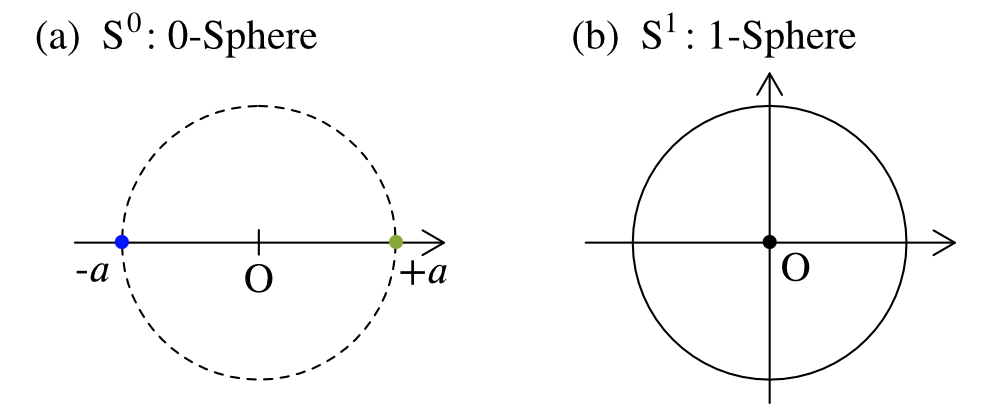
\includegraphics[scale=1]{f1_0-Sphere.png}
        \caption{\justifying $(\bm{\mathrm{a}})$ a 0-sphere $(\bm{\mathrm{b}})$ a 1-sphere. The 0-sphere consists of two points. In this paper, it illustrated in the blue and green dots. In this paper, these blue and green dots are mentioned as $\textit{the kernels}$.}
    \label{f1_0-Sphere}
\end{figure}




\subsection{Thermal energy gradient caused by two kernels}
\label{sec:ThermalEnergyGradient}

The Appendix quotes from the paper~\cite{Hanamura2018} on how the energy gradient arises from two kernels. To maintain the law of conservation of energy, we take each of the two kernels or bare electrons as a thermal potential energy. These two kernels act as both emitters and absorbers in turn. To meet the requirements for simultaneous emission and absorption, assign $T_{\mathrm{e1}}$ and $T_{\mathrm{e2}}$, as follows; 

\begin{equation}
    \begin{split}
        (Oscillator \ 1): T_{\mathrm{e1}}
            &= E_{0} \cos^{4} \left( \frac{\omega t}{2} \right) , \\
        (Oscillator \ 2): T_{\mathrm{e2}}
            &= E_{0} \sin^{4} \left( \frac{\omega t}{2} \right)
                    ,
    \label{e3_Oscillators_Te1_Te2}
    \end{split}
\end{equation}
where $E_{0}$ is the ground state of quantised energy. Set the two electrons as paired oscillators with $T_{\mathrm{e1}}$ = $E_{0} \cos^{4} \omega t /2$ and $T_{\mathrm{e2}}$ = $E_{0} \sin^{4} \omega t /2$. The temperature gradient between the two kernels is calculated as,

    \begin{equation}
            \mathrm{grad} \ T_{\mathrm{e}} = \mathrm{grad} \ ( T_{\mathrm{e2}} - T_{\mathrm{e1}} )
            \ .
            \label{e3_k_grad_Te2-Te1}
    \end{equation}

Since the values of thermal energy at both thermal kernels vary with time, the temperature gradient changes with time. Let the previous $\omega t$ is $\theta$,

\begin{align}
    \mathrm{grad} \ T_{\mathrm{e1}}
                &= \frac{d}{d \theta} \left( E_{0} \cos^{4} \left( \frac{\theta}{2} \right) \right) \notag \\
        &= - 2 E_{0} \cos^{3} \left( \frac{\theta}{2} \right) \sin \left( \frac{\theta}{2} \right)
        \ .
        \label{e3_gradT_e1}
\end{align}

\begin{align}
    \mathrm{grad} \ T_{\mathrm{e2}}
        &= \frac{d}{d \theta} \left( E_{0} \sin^{4} \left( \frac{\theta}{2} \right) \right) \notag \\
        &=   2 E_{0} \cos \left( \frac{\theta}{2} \right) \sin^{3} \left( \frac{\theta}{2} \right)
        \ .
        \label{e3_gradT_e2}
\end{align}        
$\mathrm{grad} \ T_{\mathrm{e1}}$ and $\mathrm{grad} \ T_{\mathrm{e2}}$ include only time derivative terms; their space derivatives are zero, because the kernels do not change in position with time. That is,

        \begin{align}
            \mathrm{grad} \ (T_{\mathrm{e2}} - T_{\mathrm{e1}})
                &= 2 E_{0} \cos \left( \frac{\theta}{2} \right) \sin^{3} \left( \frac{\theta}{2} \right) \notag \\
                & \quad + 2 E_{0} \cos^{3} \left( \frac{\theta}{2} \right) \sin \left( \frac{\theta}{2} \right) \notag \\
                &= 2 E_{0} \cos \left( \frac{\theta}{2} \right) \sin \left( \frac{\theta}{2} \right) \notag \\
                &= E_{0} \sin \theta
                \ .
            \label{e3_simple_harmonic_motion}
        \end{align}


Equation (\ref{e3_simple_harmonic_motion}) shows that the temperature gradient between $\mathrm{grad} \ T_{\mathrm{e1}}$ and $\mathrm{grad} \ T_{\mathrm{e2}}$ produces a force $\bm{\mathrm{F}}$. The force drives the velocity of the virtual photon along with simple harmonic motion. On the basis of the above assumption, the virtual photon swing back and force spatially between the two kernels.
    
Interaction between thermal and kinetic energy is essential in the 0-Sphere electron model, because the interaction between the two kinds of energy, i.e., the thermal potential energy of the spinors and the kinetic energy of the virtual photon, drives the virtual photon along with the harmonic oscillator. See yellow line on Fig.~\ref{f_appendix1}.


\begin{figure}[t!]
    \centering 
    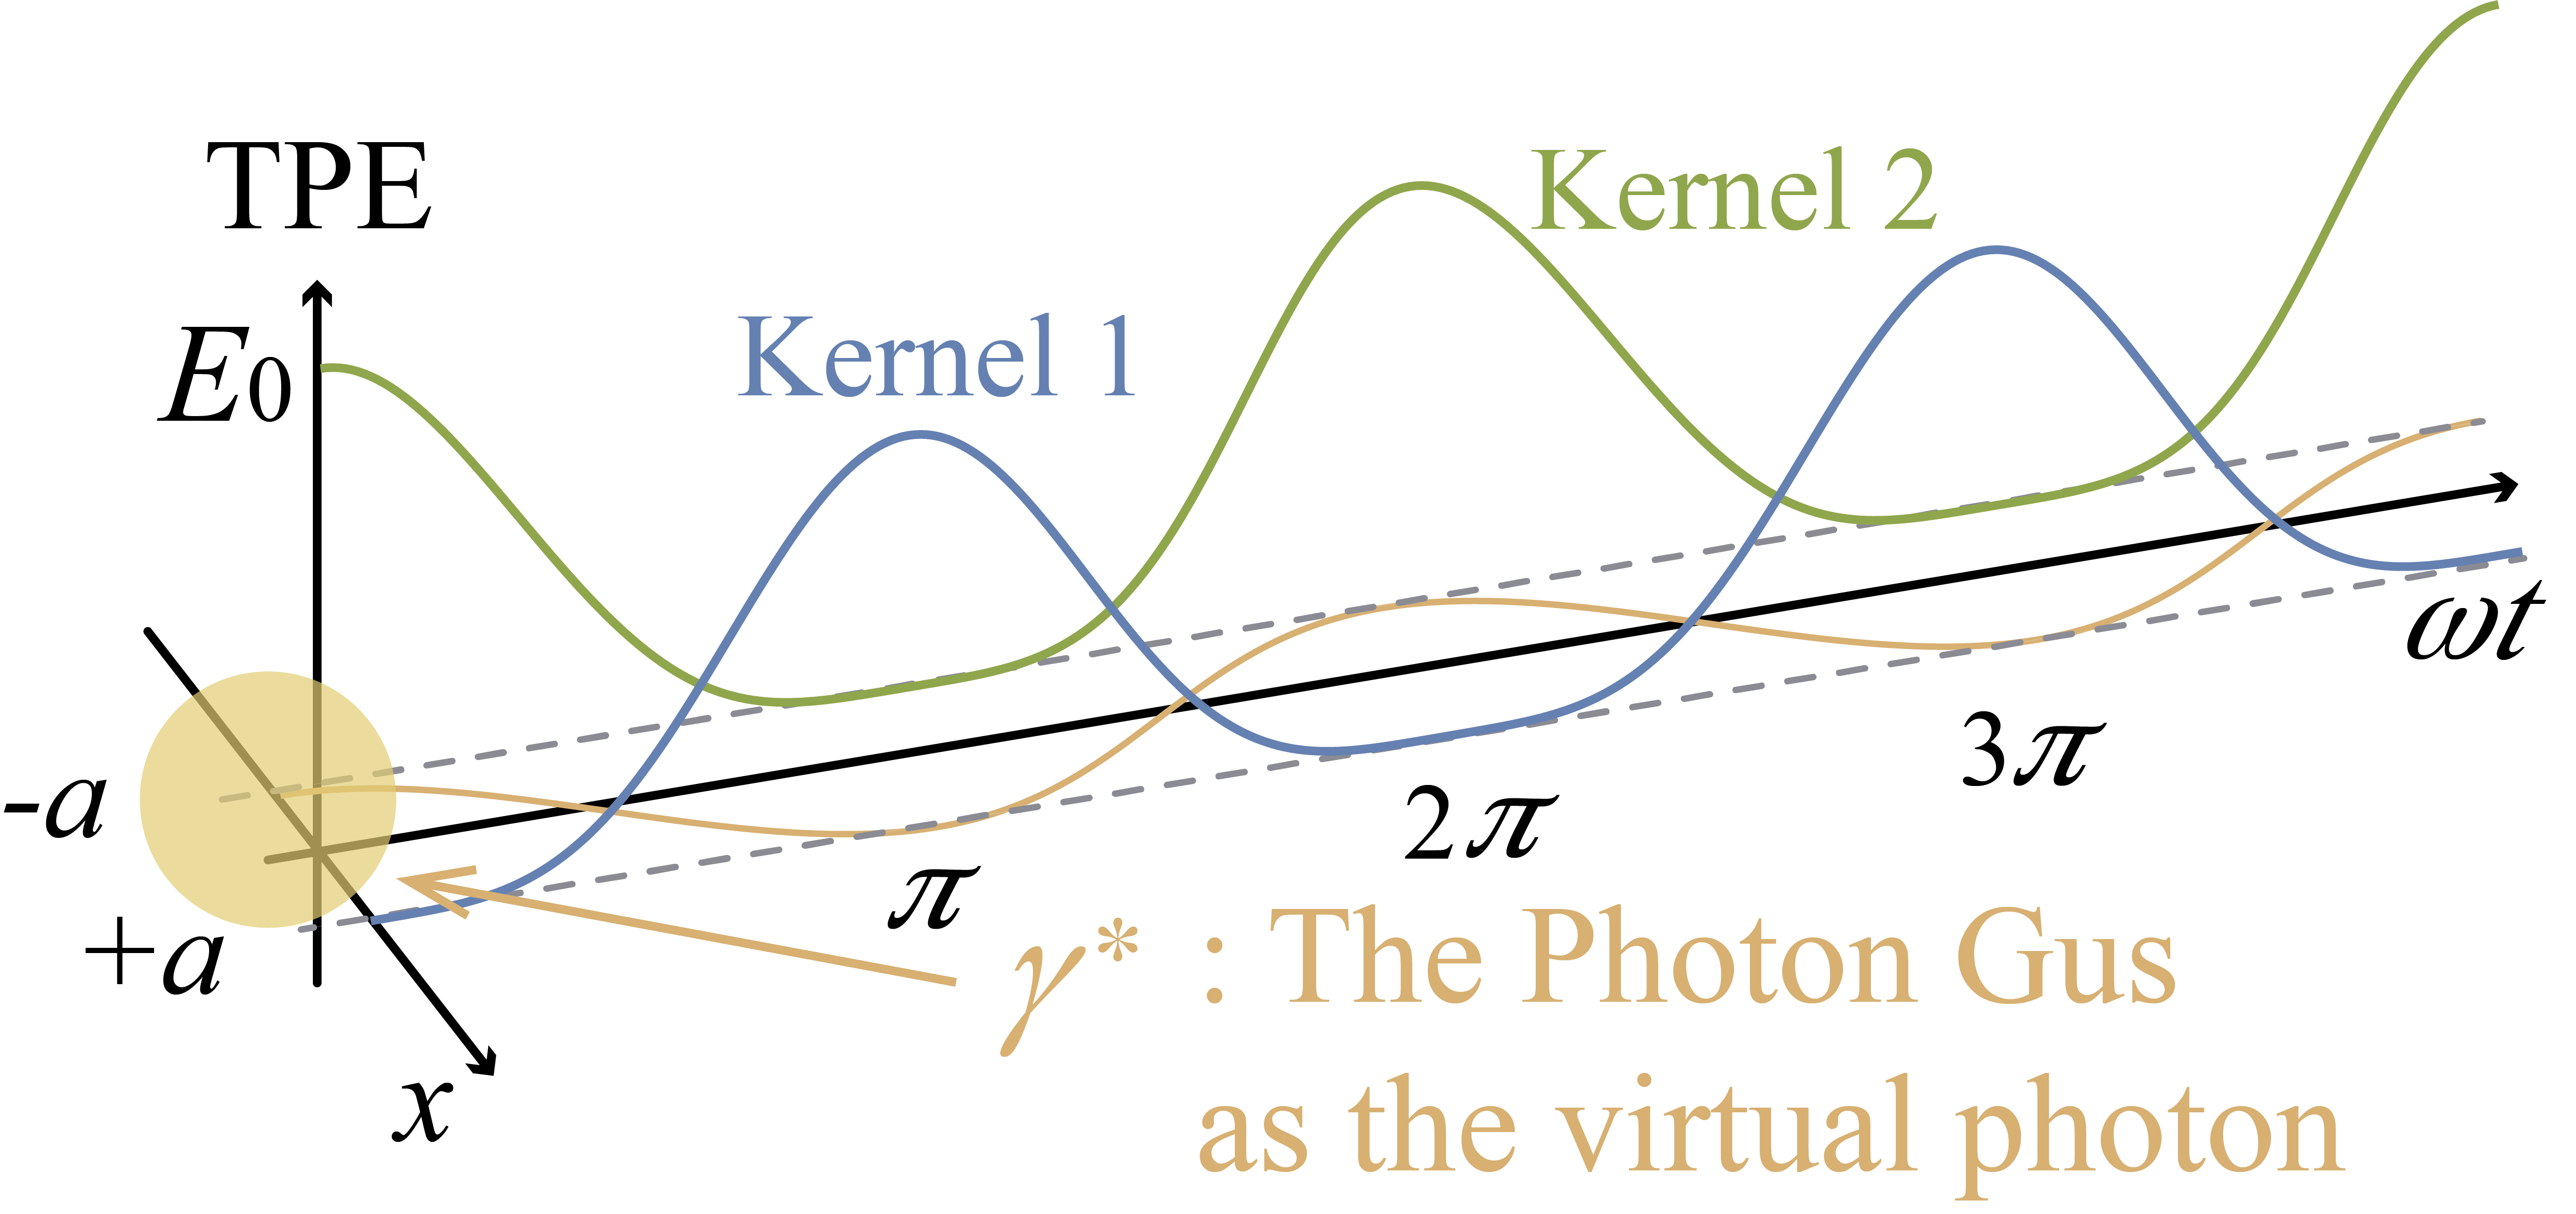
\includegraphics[scale=0.20]{f_appendix2.png}
        \caption{\justifying Behavior of the photon sphere as a spatial simple harmonic oscillator while the two kernels behave as emitters and absorbers. The blue and green dots are two kernels inside one electron. Since the equation of $ Kernel1 + Kernel2 + \gamma^{*}_{\mathrm{Kinetic.E}} = E_{\mathrm{_0}} $, the sum of the thermal potential energy (TPE) of the two kernels and the kinetic energy of the virtual photon is constant. The energy conservation law is preserved. See paper~\cite{Hanamura2018} for details.}
    \label{f_appendix1}
\end{figure}


\end{document}

% = = * * = =  * * = = * * = = * * = = * * = = * * = = * * = = * * 



